\documentclass[twoside]{book}

% Packages required by doxygen
\usepackage{calc}
\usepackage{doxygen}
\usepackage{graphicx}
\usepackage[utf8]{inputenc}
\usepackage{makeidx}
\usepackage{multicol}
\usepackage{multirow}
\usepackage{textcomp}
\usepackage[table]{xcolor}

% Font selection
\usepackage[T1]{fontenc}
\usepackage{mathptmx}
\usepackage[scaled=.90]{helvet}
\usepackage{courier}
\usepackage{amssymb}
\usepackage{sectsty}
\renewcommand{\familydefault}{\sfdefault}
\allsectionsfont{%
  \fontseries{bc}\selectfont%
  \color{darkgray}%
}
\renewcommand{\DoxyLabelFont}{%
  \fontseries{bc}\selectfont%
  \color{darkgray}%
}

% Page & text layout
\usepackage{geometry}
\geometry{%
  a4paper,%
  top=2.5cm,%
  bottom=2.5cm,%
  left=2.5cm,%
  right=2.5cm%
}
\tolerance=750
\hfuzz=15pt
\hbadness=750
\setlength{\emergencystretch}{15pt}
\setlength{\parindent}{0cm}
\setlength{\parskip}{0.2cm}
\makeatletter
\renewcommand{\paragraph}{%
  \@startsection{paragraph}{4}{0ex}{-1.0ex}{1.0ex}{%
    \normalfont\normalsize\bfseries\SS@parafont%
  }%
}
\renewcommand{\subparagraph}{%
  \@startsection{subparagraph}{5}{0ex}{-1.0ex}{1.0ex}{%
    \normalfont\normalsize\bfseries\SS@subparafont%
  }%
}
\makeatother

% Headers & footers
\usepackage{fancyhdr}
\pagestyle{fancyplain}
\fancyhead[LE]{\fancyplain{}{\bfseries\thepage}}
\fancyhead[CE]{\fancyplain{}{}}
\fancyhead[RE]{\fancyplain{}{\bfseries\leftmark}}
\fancyhead[LO]{\fancyplain{}{\bfseries\rightmark}}
\fancyhead[CO]{\fancyplain{}{}}
\fancyhead[RO]{\fancyplain{}{\bfseries\thepage}}
\fancyfoot[LE]{\fancyplain{}{}}
\fancyfoot[CE]{\fancyplain{}{}}
\fancyfoot[RE]{\fancyplain{}{\bfseries\scriptsize Generated on Fri Dec 6 2013 20\-:39\-:03 for C\-S 340 Checkers by Doxygen }}
\fancyfoot[LO]{\fancyplain{}{\bfseries\scriptsize Generated on Fri Dec 6 2013 20\-:39\-:03 for C\-S 340 Checkers by Doxygen }}
\fancyfoot[CO]{\fancyplain{}{}}
\fancyfoot[RO]{\fancyplain{}{}}
\renewcommand{\footrulewidth}{0.4pt}
\renewcommand{\chaptermark}[1]{%
  \markboth{#1}{}%
}
\renewcommand{\sectionmark}[1]{%
  \markright{\thesection\ #1}%
}

% Indices & bibliography
\usepackage{natbib}
\usepackage[titles]{tocloft}
\setcounter{tocdepth}{3}
\setcounter{secnumdepth}{5}
\makeindex

% Hyperlinks (required, but should be loaded last)
\usepackage{ifpdf}
\ifpdf
  \usepackage[pdftex,pagebackref=true]{hyperref}
\else
  \usepackage[ps2pdf,pagebackref=true]{hyperref}
\fi
\hypersetup{%
  colorlinks=true,%
  linkcolor=blue,%
  citecolor=blue,%
  unicode%
}

% Custom commands
\newcommand{\clearemptydoublepage}{%
  \newpage{\pagestyle{empty}\cleardoublepage}%
}


%===== C O N T E N T S =====

\begin{document}

% Titlepage & ToC
\hypersetup{pageanchor=false}
\pagenumbering{roman}
\begin{titlepage}
\vspace*{7cm}
\begin{center}%
{\Large C\-S 340 Checkers \\[1ex]\large Ver. 1.\-0 }\\
\vspace*{1cm}
{\large Generated by Doxygen 1.8.5}\\
\vspace*{0.5cm}
{\small Fri Dec 6 2013 20:39:03}\\
\end{center}
\end{titlepage}
\clearemptydoublepage
\tableofcontents
\clearemptydoublepage
\pagenumbering{arabic}
\hypersetup{pageanchor=true}

%--- Begin generated contents ---
\chapter{Bug List}
\label{bug}
\hypertarget{bug}{}

\begin{DoxyRefList}
\item[\label{bug__bug000001}%
\hypertarget{bug__bug000001}{}%
File \hyperlink{ai_8cpp}{ai.cpp} ]Occasional rare bug that the game would say that it's not a player's turn, yet text version of the board would say that the turn has updated. 
\item[\label{bug__bug000002}%
\hypertarget{bug__bug000002}{}%
File \hyperlink{board_8cpp}{board.cpp} ]No bugs were found with testing.  
\item[\label{bug__bug000003}%
\hypertarget{bug__bug000003}{}%
File \hyperlink{board_8h}{board.h} ]No major bugs found. 
\item[\label{bug__bug000004}%
\hypertarget{bug__bug000004}{}%
File \hyperlink{game_8cpp}{game.cpp} ]No major bugs found other than the bug specified on the \hyperlink{ai_8cpp}{A\-I.\-cpp} file  
\item[\label{bug__bug000005}%
\hypertarget{bug__bug000005}{}%
File \hyperlink{game_8h}{game.h} ]No bugs have been spotted. 
\item[\label{bug__bug000006}%
\hypertarget{bug__bug000006}{}%
File \hyperlink{main_8cpp}{main.cpp} ]No major bugs were found upon testing  
\item[\label{bug__bug000007}%
\hypertarget{bug__bug000007}{}%
File \hyperlink{mainwindow_8cpp}{mainwindow.cpp} ]No major bugs were found upon testing 
\item[\label{bug__bug000008}%
\hypertarget{bug__bug000008}{}%
File \hyperlink{mainwindow_8h}{mainwindow.h} ]No major bugs were found upon testing 
\item[\label{bug__bug000009}%
\hypertarget{bug__bug000009}{}%
File \hyperlink{tile_8cpp}{tile.cpp} ]No major bugs were found upon testing 
\item[\label{bug__bug000010}%
\hypertarget{bug__bug000010}{}%
File \hyperlink{tile_8h}{tile.h} ]No major bugs were found upon testing
\end{DoxyRefList}
\chapter{Namespace Index}
\section{Namespace List}
Here is a list of all namespaces with brief descriptions\-:\begin{DoxyCompactList}
\item\contentsline{section}{\hyperlink{namespacestd}{std} }{\pageref{namespacestd}}{}
\item\contentsline{section}{\hyperlink{namespace_ui}{Ui} }{\pageref{namespace_ui}}{}
\end{DoxyCompactList}

\chapter{Hierarchical Index}
\section{Class Hierarchy}
This inheritance list is sorted roughly, but not completely, alphabetically\-:\begin{DoxyCompactList}
\item \contentsline{section}{A\-I\-:\-:moves}{\pageref{struct_a_i_1_1moves}}{}
\item Q\-Graphics\-Rect\-Item\begin{DoxyCompactList}
\item \contentsline{section}{tile}{\pageref{classtile}}{}
\end{DoxyCompactList}
\item Q\-Graphics\-View\begin{DoxyCompactList}
\item \contentsline{section}{Board}{\pageref{class_board}}{}
\begin{DoxyCompactList}
\item \contentsline{section}{Game}{\pageref{class_game}}{}
\begin{DoxyCompactList}
\item \contentsline{section}{A\-I}{\pageref{class_a_i}}{}
\end{DoxyCompactList}
\end{DoxyCompactList}
\end{DoxyCompactList}
\item Q\-Main\-Window\begin{DoxyCompactList}
\item \contentsline{section}{Main\-Window}{\pageref{class_main_window}}{}
\end{DoxyCompactList}
\item \contentsline{section}{sq}{\pageref{structsq}}{}
\end{DoxyCompactList}

\chapter{Class Index}
\section{Class List}
Here are the classes, structs, unions and interfaces with brief descriptions\-:\begin{DoxyCompactList}
\item\contentsline{section}{\hyperlink{class_a_i}{A\-I} \\*The \hyperlink{class_a_i}{A\-I} class }{\pageref{class_a_i}}{}
\item\contentsline{section}{\hyperlink{class_board}{Board} }{\pageref{class_board}}{}
\item\contentsline{section}{\hyperlink{class_game}{Game} }{\pageref{class_game}}{}
\item\contentsline{section}{\hyperlink{class_main_window}{Main\-Window} \\*The \hyperlink{class_main_window}{Main\-Window} class The \hyperlink{class_main_window}{Main\-Window} class inherits the Q\-Main\-Window public class }{\pageref{class_main_window}}{}
\item\contentsline{section}{\hyperlink{struct_a_i_1_1moves}{A\-I\-::moves} \\*The moves struct \begin{DoxyVerb} contains the constant character values of the currentPosition, the newPositions, and the number of jumps\end{DoxyVerb}
 }{\pageref{struct_a_i_1_1moves}}{}
\item\contentsline{section}{\hyperlink{structsq}{sq} \\*The color enum

A structure containing the values of a square, which include its x and y position and the color of the square }{\pageref{structsq}}{}
\item\contentsline{section}{\hyperlink{classtile}{tile} }{\pageref{classtile}}{}
\end{DoxyCompactList}

\chapter{File Index}
\section{File List}
Here is a list of all files with brief descriptions\-:\begin{DoxyCompactList}
\item\contentsline{section}{340\-Checkers/\hyperlink{ai_8cpp}{ai.\-cpp} }{\pageref{ai_8cpp}}{}
\item\contentsline{section}{340\-Checkers/\hyperlink{ai_8h}{ai.\-h} }{\pageref{ai_8h}}{}
\item\contentsline{section}{340\-Checkers/\hyperlink{board_8cpp}{board.\-cpp} }{\pageref{board_8cpp}}{}
\item\contentsline{section}{340\-Checkers/\hyperlink{board_8h}{board.\-h} }{\pageref{board_8h}}{}
\item\contentsline{section}{340\-Checkers/\hyperlink{game_8cpp}{game.\-cpp} \\*\hyperlink{class_game}{Game} Logic implementation }{\pageref{game_8cpp}}{}
\item\contentsline{section}{340\-Checkers/\hyperlink{game_8h}{game.\-h} }{\pageref{game_8h}}{}
\item\contentsline{section}{340\-Checkers/\hyperlink{main_8cpp}{main.\-cpp} \\*This is the main class that starts the application }{\pageref{main_8cpp}}{}
\item\contentsline{section}{340\-Checkers/\hyperlink{mainwindow_8cpp}{mainwindow.\-cpp} }{\pageref{mainwindow_8cpp}}{}
\item\contentsline{section}{340\-Checkers/\hyperlink{mainwindow_8h}{mainwindow.\-h} }{\pageref{mainwindow_8h}}{}
\item\contentsline{section}{340\-Checkers/\hyperlink{tile_8cpp}{tile.\-cpp} }{\pageref{tile_8cpp}}{}
\item\contentsline{section}{340\-Checkers/\hyperlink{tile_8h}{tile.\-h} }{\pageref{tile_8h}}{}
\end{DoxyCompactList}

\chapter{Namespace Documentation}
\hypertarget{namespacestd}{\section{std Namespace Reference}
\label{namespacestd}\index{std@{std}}
}


\subsection{Detailed Description}
namespace identifier Using the standard namespace convention for implementation simplicity.

uses the standard namespace for simplicity of implementation

using namespace identifier 
\hypertarget{namespace_ui}{\section{Ui Namespace Reference}
\label{namespace_ui}\index{Ui@{Ui}}
}


\subsection{Detailed Description}
using the namespace \hyperlink{namespace_ui}{Ui} identifier 
\chapter{Class Documentation}
\hypertarget{class_a_i}{\section{A\-I Class Reference}
\label{class_a_i}\index{A\-I@{A\-I}}
}


The \hyperlink{class_a_i}{A\-I} class.  




{\ttfamily \#include $<$ai.\-h$>$}

Inheritance diagram for A\-I\-:\begin{figure}[H]
\begin{center}
\leavevmode
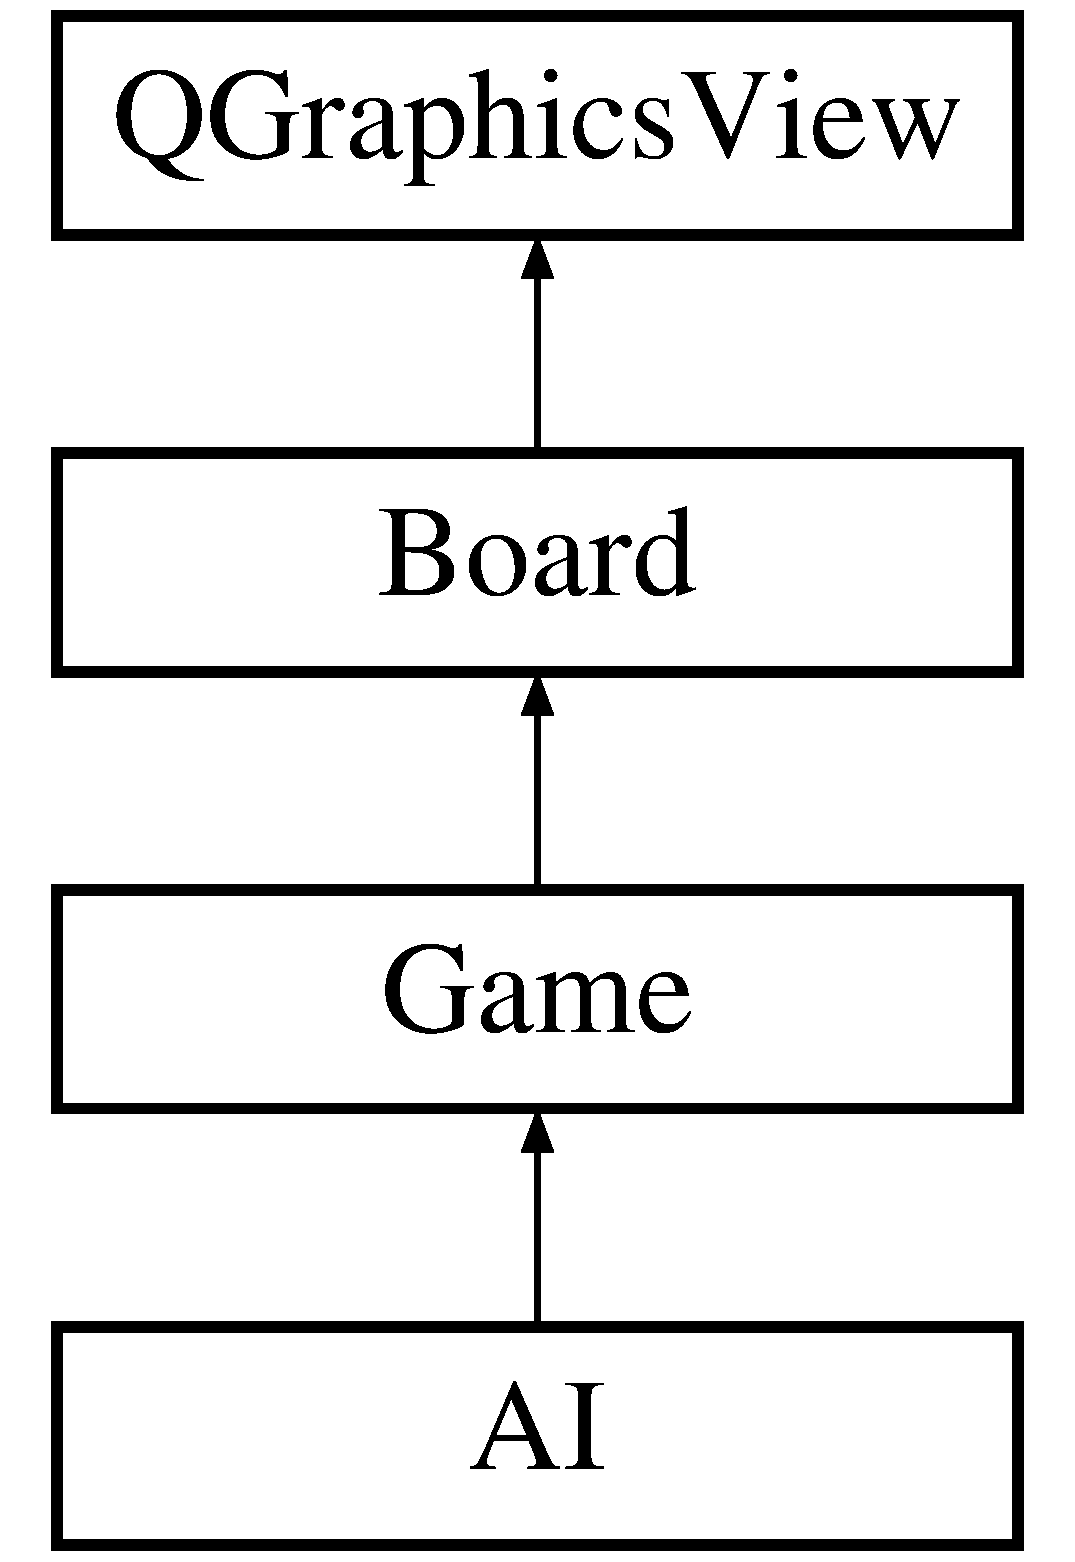
\includegraphics[height=4.000000cm]{class_a_i}
\end{center}
\end{figure}
\subsection*{Classes}
\begin{DoxyCompactItemize}
\item 
struct \hyperlink{struct_a_i_1_1moves}{moves}
\begin{DoxyCompactList}\small\item\em The moves struct \begin{DoxyVerb} contains the constant character values of the currentPosition, the newPositions, and the number of jumps\end{DoxyVerb}
. \end{DoxyCompactList}\end{DoxyCompactItemize}
\subsection*{Public Member Functions}
\begin{DoxyCompactItemize}
\item 
\hyperlink{class_a_i_a64ec60281e9eb8496f16525615db54b7}{A\-I} ()
\begin{DoxyCompactList}\small\item\em \hyperlink{class_a_i_a64ec60281e9eb8496f16525615db54b7}{A\-I\-::\-A\-I}. \end{DoxyCompactList}\item 
void \hyperlink{class_a_i_a8a7ea06489e3e3dfffbb25fbe384c205}{check\-All\-Computer\-Moves} ()
\begin{DoxyCompactList}\small\item\em \hyperlink{class_a_i_a8a7ea06489e3e3dfffbb25fbe384c205}{A\-I\-::check\-All\-Computer\-Moves} This is a method that checks all possible moves for the computer. \end{DoxyCompactList}\item 
char \hyperlink{class_a_i_aab57c3d86a7f49616d9ddeefc6978e05}{convert\-Int\-To\-Char} (int num)
\begin{DoxyCompactList}\small\item\em \hyperlink{class_a_i_aab57c3d86a7f49616d9ddeefc6978e05}{A\-I\-::convert\-Int\-To\-Char} This converts an integer to the corresponding character on the board. \end{DoxyCompactList}\item 
string \hyperlink{class_a_i_af048f2550307ee0ff15709d8e1b452b2}{decider} ()
\begin{DoxyCompactList}\small\item\em \hyperlink{class_a_i_af048f2550307ee0ff15709d8e1b452b2}{A\-I\-::decider} This is what allows the \hyperlink{class_a_i}{A\-I} to decide which move it should take. \end{DoxyCompactList}\item 
void \hyperlink{class_a_i_ae19027dd80147020d2aa55fbae3113b3}{remove\-Data} ()
\begin{DoxyCompactList}\small\item\em \hyperlink{class_a_i_ae19027dd80147020d2aa55fbae3113b3}{A\-I\-::remove\-Data} Removes the data from move\-Available, which clears the data to get newer information for a future move. \end{DoxyCompactList}\end{DoxyCompactItemize}
\subsection*{Public Attributes}
\begin{DoxyCompactItemize}
\item 
vector$<$ \hyperlink{struct_a_i_1_1moves}{moves} $>$ \hyperlink{class_a_i_afbd7b83dc6eb3a47fcde351e9a6eb651}{available\-Moves}
\end{DoxyCompactItemize}
\subsection*{Additional Inherited Members}


\subsection{Detailed Description}
The \hyperlink{class_a_i}{A\-I} class. 

\subsection{Constructor \& Destructor Documentation}
\hypertarget{class_a_i_a64ec60281e9eb8496f16525615db54b7}{\index{A\-I@{A\-I}!A\-I@{A\-I}}
\index{A\-I@{A\-I}!AI@{A\-I}}
\subsubsection[{A\-I}]{\setlength{\rightskip}{0pt plus 5cm}A\-I\-::\-A\-I (
\begin{DoxyParamCaption}
{}
\end{DoxyParamCaption}
)}}\label{class_a_i_a64ec60281e9eb8496f16525615db54b7}


\hyperlink{class_a_i_a64ec60281e9eb8496f16525615db54b7}{A\-I\-::\-A\-I}. 



\subsection{Member Function Documentation}
\hypertarget{class_a_i_a8a7ea06489e3e3dfffbb25fbe384c205}{\index{A\-I@{A\-I}!check\-All\-Computer\-Moves@{check\-All\-Computer\-Moves}}
\index{check\-All\-Computer\-Moves@{check\-All\-Computer\-Moves}!AI@{A\-I}}
\subsubsection[{check\-All\-Computer\-Moves}]{\setlength{\rightskip}{0pt plus 5cm}void A\-I\-::check\-All\-Computer\-Moves (
\begin{DoxyParamCaption}
{}
\end{DoxyParamCaption}
)}}\label{class_a_i_a8a7ea06489e3e3dfffbb25fbe384c205}


\hyperlink{class_a_i_a8a7ea06489e3e3dfffbb25fbe384c205}{A\-I\-::check\-All\-Computer\-Moves} This is a method that checks all possible moves for the computer. 

\hypertarget{class_a_i_aab57c3d86a7f49616d9ddeefc6978e05}{\index{A\-I@{A\-I}!convert\-Int\-To\-Char@{convert\-Int\-To\-Char}}
\index{convert\-Int\-To\-Char@{convert\-Int\-To\-Char}!AI@{A\-I}}
\subsubsection[{convert\-Int\-To\-Char}]{\setlength{\rightskip}{0pt plus 5cm}char A\-I\-::convert\-Int\-To\-Char (
\begin{DoxyParamCaption}
\item[{int}]{num}
\end{DoxyParamCaption}
)}}\label{class_a_i_aab57c3d86a7f49616d9ddeefc6978e05}


\hyperlink{class_a_i_aab57c3d86a7f49616d9ddeefc6978e05}{A\-I\-::convert\-Int\-To\-Char} This converts an integer to the corresponding character on the board. 


\begin{DoxyParams}{Parameters}
{\em num} & \\
\hline
\end{DoxyParams}
\begin{DoxyReturn}{Returns}

\end{DoxyReturn}
\hypertarget{class_a_i_af048f2550307ee0ff15709d8e1b452b2}{\index{A\-I@{A\-I}!decider@{decider}}
\index{decider@{decider}!AI@{A\-I}}
\subsubsection[{decider}]{\setlength{\rightskip}{0pt plus 5cm}string A\-I\-::decider (
\begin{DoxyParamCaption}
{}
\end{DoxyParamCaption}
)}}\label{class_a_i_af048f2550307ee0ff15709d8e1b452b2}


\hyperlink{class_a_i_af048f2550307ee0ff15709d8e1b452b2}{A\-I\-::decider} This is what allows the \hyperlink{class_a_i}{A\-I} to decide which move it should take. 

\begin{DoxyReturn}{Returns}

\end{DoxyReturn}
\hypertarget{class_a_i_ae19027dd80147020d2aa55fbae3113b3}{\index{A\-I@{A\-I}!remove\-Data@{remove\-Data}}
\index{remove\-Data@{remove\-Data}!AI@{A\-I}}
\subsubsection[{remove\-Data}]{\setlength{\rightskip}{0pt plus 5cm}void A\-I\-::remove\-Data (
\begin{DoxyParamCaption}
{}
\end{DoxyParamCaption}
)}}\label{class_a_i_ae19027dd80147020d2aa55fbae3113b3}


\hyperlink{class_a_i_ae19027dd80147020d2aa55fbae3113b3}{A\-I\-::remove\-Data} Removes the data from move\-Available, which clears the data to get newer information for a future move. 



\subsection{Member Data Documentation}
\hypertarget{class_a_i_afbd7b83dc6eb3a47fcde351e9a6eb651}{\index{A\-I@{A\-I}!available\-Moves@{available\-Moves}}
\index{available\-Moves@{available\-Moves}!AI@{A\-I}}
\subsubsection[{available\-Moves}]{\setlength{\rightskip}{0pt plus 5cm}vector$<${\bf moves}$>$ A\-I\-::available\-Moves}}\label{class_a_i_afbd7b83dc6eb3a47fcde351e9a6eb651}


The documentation for this class was generated from the following files\-:\begin{DoxyCompactItemize}
\item 
\hyperlink{ai_8h}{ai.\-h}\item 
\hyperlink{ai_8cpp}{ai.\-cpp}\end{DoxyCompactItemize}

\hypertarget{class_board}{\section{Board Class Reference}
\label{class_board}\index{Board@{Board}}
}


{\ttfamily \#include $<$board.\-h$>$}

Inheritance diagram for Board\-:\begin{figure}[H]
\begin{center}
\leavevmode
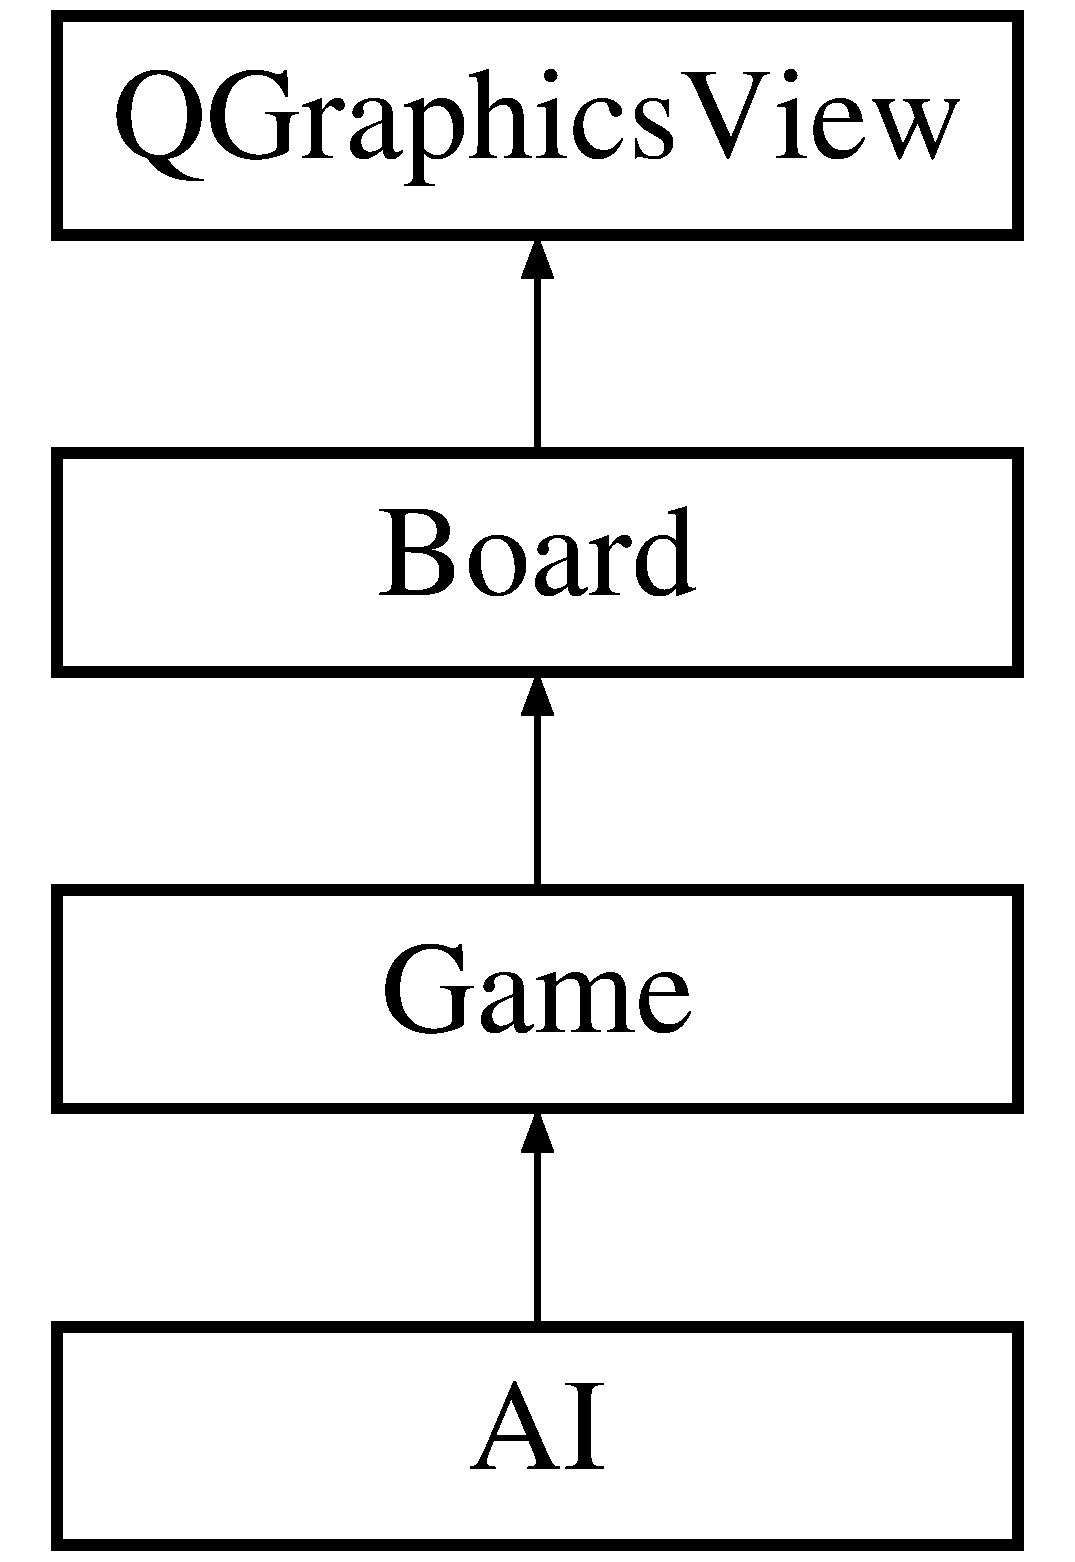
\includegraphics[height=4.000000cm]{class_board}
\end{center}
\end{figure}
\subsection*{Public Member Functions}
\begin{DoxyCompactItemize}
\item 
\hyperlink{class_board_a9ee491d4fea680cf69b033374a9fdfcb}{Board} ()
\begin{DoxyCompactList}\small\item\em \hyperlink{class_board_a9ee491d4fea680cf69b033374a9fdfcb}{Board\-::\-Board} A \hyperlink{class_board}{Board} constructor that initializes the board. \end{DoxyCompactList}\item 
void \hyperlink{class_board_ad3e7c6a4070b1dac5b124a550fa0a6fc}{display\-Board} (int player1\-Score, int player2\-Score)
\begin{DoxyCompactList}\small\item\em \hyperlink{class_board_ad3e7c6a4070b1dac5b124a550fa0a6fc}{Board\-::display\-Board} Displays the current \hyperlink{class_board}{Board} with both players' scores (the remaining pieces) \end{DoxyCompactList}\item 
void \hyperlink{class_board_a799c675452ae1a6d3dd6b2058c88f92a}{add\-Grid} (Q\-Graphics\-Scene $\ast$scene)
\begin{DoxyCompactList}\small\item\em \hyperlink{class_board_a799c675452ae1a6d3dd6b2058c88f92a}{Board\-::add\-Grid} This will generate the graphical grid and create a G\-U\-I with the visual board. \end{DoxyCompactList}\item 
void \hyperlink{class_board_a964d67ddc797487f1a018e4c7cd82075}{update\-Grid} (Q\-Graphics\-Scene $\ast$scene)
\begin{DoxyCompactList}\small\item\em \hyperlink{class_board_a964d67ddc797487f1a018e4c7cd82075}{Board\-::update\-Grid} Updates the grid with the current turn and pieces remaining on the board. \end{DoxyCompactList}\end{DoxyCompactItemize}
\subsection*{Public Attributes}
\begin{DoxyCompactItemize}
\item 
\hyperlink{structsq}{sq} \hyperlink{class_board_acd3e1340f25b2d2371d8a2862e473b15}{tiles} \mbox{[}8\mbox{]}\mbox{[}8\mbox{]}
\item 
char \hyperlink{class_board_a6e32218e7d8adc57f9d414836d135d96}{board} \mbox{[}\hyperlink{class_board_a3b3d4827430812c8849610301dbf91f3}{B\-O\-A\-R\-D\-\_\-\-L\-E\-N\-G\-T\-H}\mbox{]}\mbox{[}\hyperlink{class_board_a3b3d4827430812c8849610301dbf91f3}{B\-O\-A\-R\-D\-\_\-\-L\-E\-N\-G\-T\-H}\mbox{]}
\end{DoxyCompactItemize}
\subsection*{Static Public Attributes}
\begin{DoxyCompactItemize}
\item 
static const int \hyperlink{class_board_a3b3d4827430812c8849610301dbf91f3}{B\-O\-A\-R\-D\-\_\-\-L\-E\-N\-G\-T\-H} = 8
\end{DoxyCompactItemize}


\subsection{Constructor \& Destructor Documentation}
\hypertarget{class_board_a9ee491d4fea680cf69b033374a9fdfcb}{\index{Board@{Board}!Board@{Board}}
\index{Board@{Board}!Board@{Board}}
\subsubsection[{Board}]{\setlength{\rightskip}{0pt plus 5cm}Board\-::\-Board (
\begin{DoxyParamCaption}
{}
\end{DoxyParamCaption}
)}}\label{class_board_a9ee491d4fea680cf69b033374a9fdfcb}


\hyperlink{class_board_a9ee491d4fea680cf69b033374a9fdfcb}{Board\-::\-Board} A \hyperlink{class_board}{Board} constructor that initializes the board. 



\subsection{Member Function Documentation}
\hypertarget{class_board_a799c675452ae1a6d3dd6b2058c88f92a}{\index{Board@{Board}!add\-Grid@{add\-Grid}}
\index{add\-Grid@{add\-Grid}!Board@{Board}}
\subsubsection[{add\-Grid}]{\setlength{\rightskip}{0pt plus 5cm}void Board\-::add\-Grid (
\begin{DoxyParamCaption}
\item[{Q\-Graphics\-Scene $\ast$}]{scene}
\end{DoxyParamCaption}
)}}\label{class_board_a799c675452ae1a6d3dd6b2058c88f92a}


\hyperlink{class_board_a799c675452ae1a6d3dd6b2058c88f92a}{Board\-::add\-Grid} This will generate the graphical grid and create a G\-U\-I with the visual board. 


\begin{DoxyParams}{Parameters}
{\em scene} & \\
\hline
\end{DoxyParams}
\hypertarget{class_board_ad3e7c6a4070b1dac5b124a550fa0a6fc}{\index{Board@{Board}!display\-Board@{display\-Board}}
\index{display\-Board@{display\-Board}!Board@{Board}}
\subsubsection[{display\-Board}]{\setlength{\rightskip}{0pt plus 5cm}void Board\-::display\-Board (
\begin{DoxyParamCaption}
\item[{int}]{player1\-Score, }
\item[{int}]{player2\-Score}
\end{DoxyParamCaption}
)}}\label{class_board_ad3e7c6a4070b1dac5b124a550fa0a6fc}


\hyperlink{class_board_ad3e7c6a4070b1dac5b124a550fa0a6fc}{Board\-::display\-Board} Displays the current \hyperlink{class_board}{Board} with both players' scores (the remaining pieces) 


\begin{DoxyParams}{Parameters}
{\em player1\-Score} & \\
\hline
{\em player2\-Score} & \\
\hline
\end{DoxyParams}
\hypertarget{class_board_a964d67ddc797487f1a018e4c7cd82075}{\index{Board@{Board}!update\-Grid@{update\-Grid}}
\index{update\-Grid@{update\-Grid}!Board@{Board}}
\subsubsection[{update\-Grid}]{\setlength{\rightskip}{0pt plus 5cm}void Board\-::update\-Grid (
\begin{DoxyParamCaption}
\item[{Q\-Graphics\-Scene $\ast$}]{scene}
\end{DoxyParamCaption}
)}}\label{class_board_a964d67ddc797487f1a018e4c7cd82075}


\hyperlink{class_board_a964d67ddc797487f1a018e4c7cd82075}{Board\-::update\-Grid} Updates the grid with the current turn and pieces remaining on the board. 


\begin{DoxyParams}{Parameters}
{\em scene} & \\
\hline
\end{DoxyParams}


\subsection{Member Data Documentation}
\hypertarget{class_board_a6e32218e7d8adc57f9d414836d135d96}{\index{Board@{Board}!board@{board}}
\index{board@{board}!Board@{Board}}
\subsubsection[{board}]{\setlength{\rightskip}{0pt plus 5cm}char Board\-::board\mbox{[}{\bf B\-O\-A\-R\-D\-\_\-\-L\-E\-N\-G\-T\-H}\mbox{]}\mbox{[}{\bf B\-O\-A\-R\-D\-\_\-\-L\-E\-N\-G\-T\-H}\mbox{]}}}\label{class_board_a6e32218e7d8adc57f9d414836d135d96}
\hypertarget{class_board_a3b3d4827430812c8849610301dbf91f3}{\index{Board@{Board}!B\-O\-A\-R\-D\-\_\-\-L\-E\-N\-G\-T\-H@{B\-O\-A\-R\-D\-\_\-\-L\-E\-N\-G\-T\-H}}
\index{B\-O\-A\-R\-D\-\_\-\-L\-E\-N\-G\-T\-H@{B\-O\-A\-R\-D\-\_\-\-L\-E\-N\-G\-T\-H}!Board@{Board}}
\subsubsection[{B\-O\-A\-R\-D\-\_\-\-L\-E\-N\-G\-T\-H}]{\setlength{\rightskip}{0pt plus 5cm}const int Board\-::\-B\-O\-A\-R\-D\-\_\-\-L\-E\-N\-G\-T\-H = 8\hspace{0.3cm}{\ttfamily [static]}}}\label{class_board_a3b3d4827430812c8849610301dbf91f3}
\hypertarget{class_board_acd3e1340f25b2d2371d8a2862e473b15}{\index{Board@{Board}!tiles@{tiles}}
\index{tiles@{tiles}!Board@{Board}}
\subsubsection[{tiles}]{\setlength{\rightskip}{0pt plus 5cm}{\bf sq} Board\-::tiles\mbox{[}8\mbox{]}\mbox{[}8\mbox{]}}}\label{class_board_acd3e1340f25b2d2371d8a2862e473b15}


The documentation for this class was generated from the following files\-:\begin{DoxyCompactItemize}
\item 
\hyperlink{board_8h}{board.\-h}\item 
\hyperlink{board_8cpp}{board.\-cpp}\end{DoxyCompactItemize}

\hypertarget{class_game}{\section{Game Class Reference}
\label{class_game}\index{Game@{Game}}
}


{\ttfamily \#include $<$game.\-h$>$}

Inheritance diagram for Game\-:\begin{figure}[H]
\begin{center}
\leavevmode
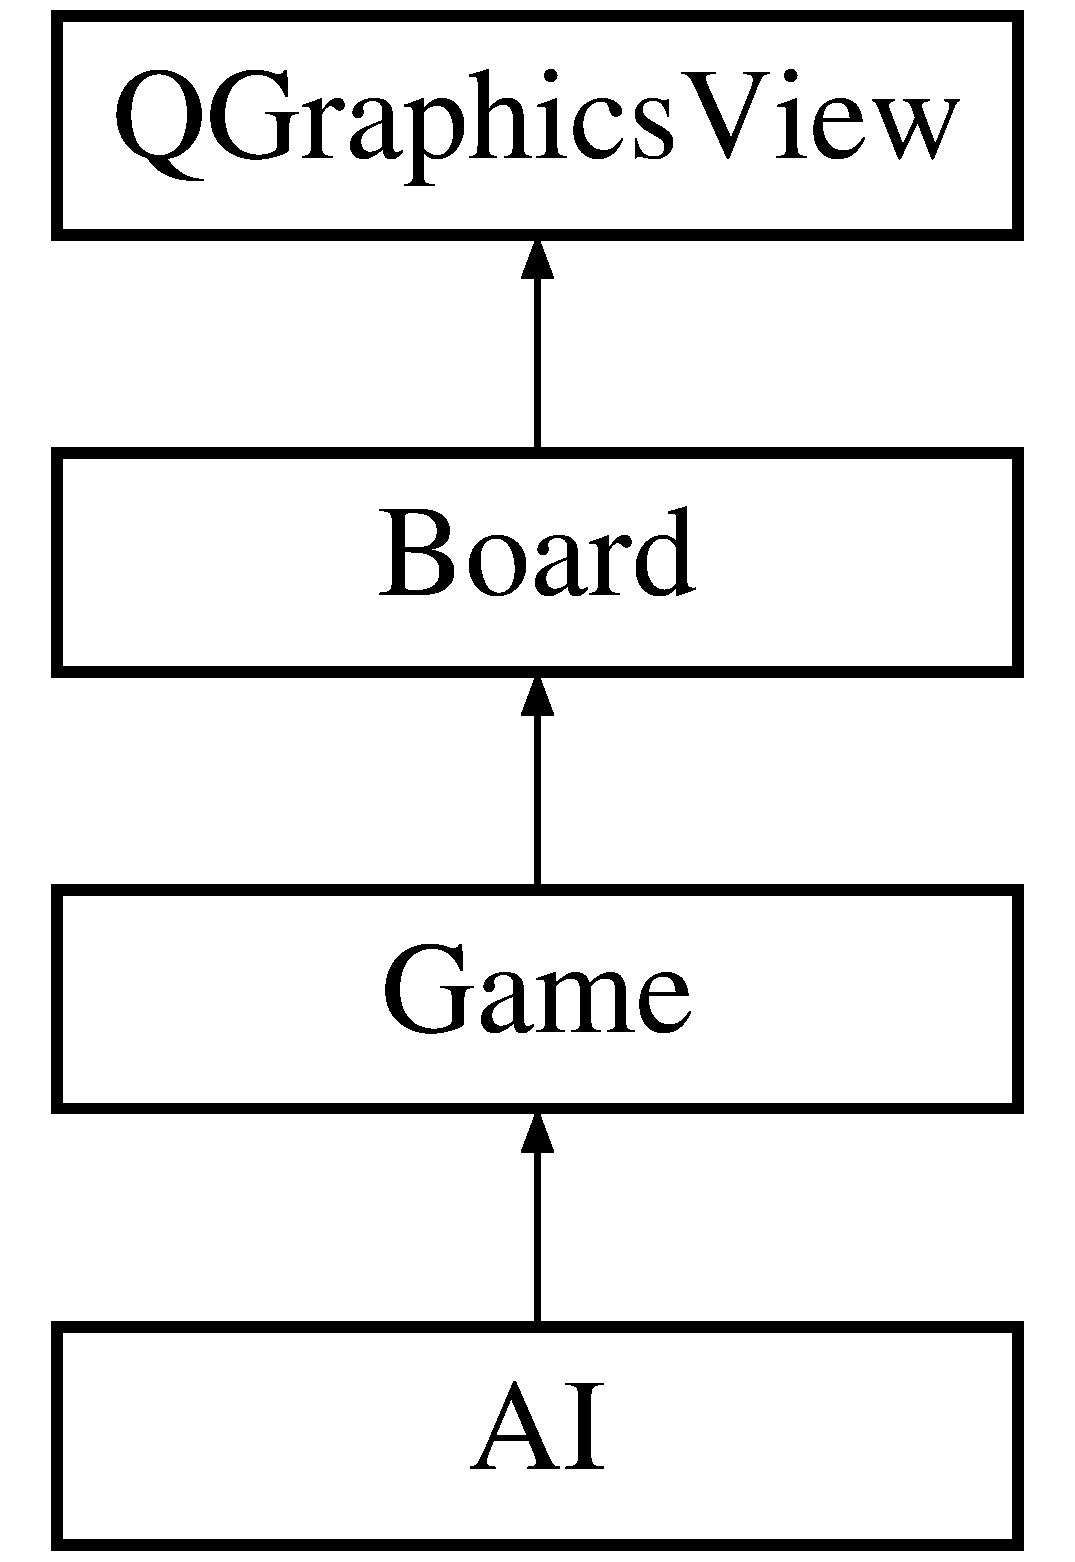
\includegraphics[height=4.000000cm]{class_game}
\end{center}
\end{figure}
\subsection*{Public Member Functions}
\begin{DoxyCompactItemize}
\item 
\hyperlink{class_game_ad59df6562a58a614fda24622d3715b65}{Game} ()
\item 
bool \hyperlink{class_game_a85a222741ee55b73e12cca53487f0540}{make\-A\-Move} (int player, char $\ast$piece\-To\-Move, char $\ast$move\-To)
\item 
int \hyperlink{class_game_a708211cd7858e1628cef1b98e2712797}{convert\-Char\-Dimension\-To\-Int} (char second\-Dimension)
\begin{DoxyCompactList}\small\item\em \hyperlink{class_game_a708211cd7858e1628cef1b98e2712797}{Game\-::convert\-Char\-Dimension\-To\-Int} This method converts the second dimension from a character to an integer. \end{DoxyCompactList}\item 
bool \hyperlink{class_game_ab049a593d3f303c4b090f3e25cbf1056}{move\-Regular\-P1\-Up} (int new\-First\-Dimension, int current\-First\-Dimension, int new\-Second\-Dimension, int current\-Second\-Dimension)
\begin{DoxyCompactList}\small\item\em \hyperlink{class_game_ab049a593d3f303c4b090f3e25cbf1056}{Game\-::move\-Regular\-P1\-Up} Moves the regular piece for player 1 up the board. \end{DoxyCompactList}\item 
bool \hyperlink{class_game_aff639012e102ce42f09306bbf580c391}{move\-King\-P1} (int new\-First\-Dimension, int current\-First\-Dimension, int new\-Second\-Dimension, int current\-Second\-Dimension)
\begin{DoxyCompactList}\small\item\em \hyperlink{class_game_aff639012e102ce42f09306bbf580c391}{Game\-::move\-King\-P1} Moves the player 1 King piece. \end{DoxyCompactList}\item 
bool \hyperlink{class_game_aad3a58175a91d8235771707620846429}{move\-Regular\-P2\-Down} (int new\-First\-Dimension, int current\-First\-Dimension, int new\-Second\-Dimension, int current\-Second\-Dimension)
\begin{DoxyCompactList}\small\item\em \hyperlink{class_game_aad3a58175a91d8235771707620846429}{Game\-::move\-Regular\-P2\-Down} A method that moves a player 2's regular piece down the board. \end{DoxyCompactList}\item 
bool \hyperlink{class_game_ae89d9850dd157a1ace783ca8785411f3}{move\-King\-P2} (int new\-First\-Dimension, int current\-First\-Dimension, int new\-Second\-Dimension, int current\-Second\-Dimension)
\begin{DoxyCompactList}\small\item\em \hyperlink{class_game_ae89d9850dd157a1ace783ca8785411f3}{Game\-::move\-King\-P2} Moves the player 2's King piece. \end{DoxyCompactList}\item 
bool \hyperlink{class_game_a9e622f6a5fe4c04a0cf2055b3da1c2f2}{can\-Jump\-Player} (char $\ast$current\-Pos)
\begin{DoxyCompactList}\small\item\em \hyperlink{class_game_a9e622f6a5fe4c04a0cf2055b3da1c2f2}{Game\-::can\-Jump\-Player} A method that checks to see if a player can jump another player. \end{DoxyCompactList}\item 
string \hyperlink{class_game_af770bb006101a532326310417011b5e6}{jump\-Pos} (char $\ast$current\-Pos)
\begin{DoxyCompactList}\small\item\em \hyperlink{class_game_af770bb006101a532326310417011b5e6}{Game\-::jump\-Pos} Checks if the player can jump another player. \end{DoxyCompactList}\item 
char \hyperlink{class_game_a6d8b525593305e2a573fc7fc13bca103}{convert\-Int\-To\-Char} (int num)
\begin{DoxyCompactList}\small\item\em \hyperlink{class_game_a6d8b525593305e2a573fc7fc13bca103}{Game\-::convert\-Int\-To\-Char} Convert an integer to a corresponding character on the board. \end{DoxyCompactList}\end{DoxyCompactItemize}
\subsection*{Public Attributes}
\begin{DoxyCompactItemize}
\item 
int \hyperlink{class_game_af6803e417a57dcf56debfd2ecdcc9661}{current\-Piece}
\item 
int \hyperlink{class_game_af0938fa4b54d37a0c3099397a58d3cd7}{current\-King\-Piece}
\item 
int \hyperlink{class_game_a54d8c544103d5721e83e75c0fb42a4a3}{player1\-Score}
\item 
int \hyperlink{class_game_a6ceb54d51da7bfd37492c3ebcea60412}{player2\-Score}
\item 
bool \hyperlink{class_game_aa7bf3272e009587fca6a67b486e27418}{another\-Jump}
\end{DoxyCompactItemize}
\subsection*{Additional Inherited Members}


\subsection{Detailed Description}


Definition at line 99 of file game.\-h.



\subsection{Constructor \& Destructor Documentation}
\hypertarget{class_game_ad59df6562a58a614fda24622d3715b65}{\index{Game@{Game}!Game@{Game}}
\index{Game@{Game}!Game@{Game}}
\subsubsection[{Game}]{\setlength{\rightskip}{0pt plus 5cm}Game\-::\-Game (
\begin{DoxyParamCaption}
{}
\end{DoxyParamCaption}
)}}\label{class_game_ad59df6562a58a614fda24622d3715b65}


Definition at line 44 of file game.\-cpp.



\subsection{Member Function Documentation}
\hypertarget{class_game_a9e622f6a5fe4c04a0cf2055b3da1c2f2}{\index{Game@{Game}!can\-Jump\-Player@{can\-Jump\-Player}}
\index{can\-Jump\-Player@{can\-Jump\-Player}!Game@{Game}}
\subsubsection[{can\-Jump\-Player}]{\setlength{\rightskip}{0pt plus 5cm}bool Game\-::can\-Jump\-Player (
\begin{DoxyParamCaption}
\item[{char $\ast$}]{current\-Pos}
\end{DoxyParamCaption}
)}}\label{class_game_a9e622f6a5fe4c04a0cf2055b3da1c2f2}


\hyperlink{class_game_a9e622f6a5fe4c04a0cf2055b3da1c2f2}{Game\-::can\-Jump\-Player} A method that checks to see if a player can jump another player. 

This method receives a parameter that tells the method what the current position is, which then the application will use to check to see if any of the adjacent pieces are enemy pieces. First the game will determine if the current piece is a King piece or a regular piece. Then, it will scan to see if there is an opponent's piece adjacent to them, meaning that there is a possibility that the player can make a jump. Once the game detects that an opponent piece is next to them, it will check the piece adjacent to the opponent piece and make sure that the piece adjacent to them is empty; bear in mind, that the application will also keep track to see if the jump is legal, that is, the piece can safely jump a player and still be within the board's dimensions. It will run the same tests for each type of piece (the P1 regular, P2 regular, P1 King, and the P2 King), where the King pieces function slightly different than the regular pieces. The King can jump in any direction, so it then has to check every adjacent piece to see if it can jump. Meanwhile, the regular pieces only need to check above them (player 1 regular) or below them (player 2 regular).


\begin{DoxyParams}{Parameters}
{\em current\-Pos} & The current position of a piece, determined by its coordinates \\
\hline
\end{DoxyParams}
\begin{DoxyReturn}{Returns}
true if there is a player and there can be a jump, otherwise it will return false 
\end{DoxyReturn}


Definition at line 775 of file game.\-cpp.

\hypertarget{class_game_a708211cd7858e1628cef1b98e2712797}{\index{Game@{Game}!convert\-Char\-Dimension\-To\-Int@{convert\-Char\-Dimension\-To\-Int}}
\index{convert\-Char\-Dimension\-To\-Int@{convert\-Char\-Dimension\-To\-Int}!Game@{Game}}
\subsubsection[{convert\-Char\-Dimension\-To\-Int}]{\setlength{\rightskip}{0pt plus 5cm}int Game\-::convert\-Char\-Dimension\-To\-Int (
\begin{DoxyParamCaption}
\item[{char}]{second\-Dimension}
\end{DoxyParamCaption}
)}}\label{class_game_a708211cd7858e1628cef1b98e2712797}


\hyperlink{class_game_a708211cd7858e1628cef1b98e2712797}{Game\-::convert\-Char\-Dimension\-To\-Int} This method converts the second dimension from a character to an integer. 

The method receives the character (the coordinate) of the board, rather the letter corresponding to 1/2 of the coordinates and will convert the value into an integer such that the application can process the information in finding out the move. 
\begin{DoxyParams}{Parameters}
{\em second\-Dimension} & a coodinate that corresponds to a move \\
\hline
\end{DoxyParams}
\begin{DoxyReturn}{Returns}
A successful conversion in processing the move of a player 
\end{DoxyReturn}


Definition at line 713 of file game.\-cpp.

\hypertarget{class_game_a6d8b525593305e2a573fc7fc13bca103}{\index{Game@{Game}!convert\-Int\-To\-Char@{convert\-Int\-To\-Char}}
\index{convert\-Int\-To\-Char@{convert\-Int\-To\-Char}!Game@{Game}}
\subsubsection[{convert\-Int\-To\-Char}]{\setlength{\rightskip}{0pt plus 5cm}char Game\-::convert\-Int\-To\-Char (
\begin{DoxyParamCaption}
\item[{int}]{num}
\end{DoxyParamCaption}
)}}\label{class_game_a6d8b525593305e2a573fc7fc13bca103}


\hyperlink{class_game_a6d8b525593305e2a573fc7fc13bca103}{Game\-::convert\-Int\-To\-Char} Convert an integer to a corresponding character on the board. 

After the game makes its computations to authenticate a valid move for a given player, the game does the move, then checks to see if a jump can be made (or has been made). Then after it finishes the calculations, it then converts the integer that was generated earlier back to its corresponding character that is part of the move coordinates when making a move. 
\begin{DoxyParams}{Parameters}
{\em num} & The number corresponding to a coordinate of a game piece \\
\hline
\end{DoxyParams}
\begin{DoxyReturn}{Returns}
the coordinate of the board for a move 
\end{DoxyReturn}


Definition at line 1380 of file game.\-cpp.

\hypertarget{class_game_af770bb006101a532326310417011b5e6}{\index{Game@{Game}!jump\-Pos@{jump\-Pos}}
\index{jump\-Pos@{jump\-Pos}!Game@{Game}}
\subsubsection[{jump\-Pos}]{\setlength{\rightskip}{0pt plus 5cm}string Game\-::jump\-Pos (
\begin{DoxyParamCaption}
\item[{char $\ast$}]{current\-Pos}
\end{DoxyParamCaption}
)}}\label{class_game_af770bb006101a532326310417011b5e6}


\hyperlink{class_game_af770bb006101a532326310417011b5e6}{Game\-::jump\-Pos} Checks if the player can jump another player. 

This method is more or less a decider that decides whether or not a player's piece can be jumped. Similar to the can\-Jump\-Player method it largely does the same checks to see if the jump that can be made is legal, and if it's legal, then the piece will jump, otherwise, it will not jump anc continue the game. This is largely used to see if another piece can be jumped after the initial jump was made. 
\begin{DoxyParams}{Parameters}
{\em current\-Pos} & The current position of a gamepiece \\
\hline
\end{DoxyParams}
\begin{DoxyReturn}{Returns}
the new position of the current piece since it jumped, and it must relay the information back to the board. 
\end{DoxyReturn}


Definition at line 1054 of file game.\-cpp.

\hypertarget{class_game_a85a222741ee55b73e12cca53487f0540}{\index{Game@{Game}!make\-A\-Move@{make\-A\-Move}}
\index{make\-A\-Move@{make\-A\-Move}!Game@{Game}}
\subsubsection[{make\-A\-Move}]{\setlength{\rightskip}{0pt plus 5cm}bool Game\-::make\-A\-Move (
\begin{DoxyParamCaption}
\item[{int}]{player, }
\item[{char $\ast$}]{piece\-To\-Move, }
\item[{char $\ast$}]{move\-To}
\end{DoxyParamCaption}
)}}\label{class_game_a85a222741ee55b73e12cca53487f0540}


Definition at line 74 of file game.\-cpp.

\hypertarget{class_game_aff639012e102ce42f09306bbf580c391}{\index{Game@{Game}!move\-King\-P1@{move\-King\-P1}}
\index{move\-King\-P1@{move\-King\-P1}!Game@{Game}}
\subsubsection[{move\-King\-P1}]{\setlength{\rightskip}{0pt plus 5cm}bool Game\-::move\-King\-P1 (
\begin{DoxyParamCaption}
\item[{int}]{new\-First\-Dimension, }
\item[{int}]{current\-First\-Dimension, }
\item[{int}]{new\-Second\-Dimension, }
\item[{int}]{current\-Second\-Dimension}
\end{DoxyParamCaption}
)}}\label{class_game_aff639012e102ce42f09306bbf580c391}


\hyperlink{class_game_aff639012e102ce42f09306bbf580c391}{Game\-::move\-King\-P1} Moves the player 1 King piece. 

This method is called upon the move\-A\-Move method. What happens is that the game runs a series of error checks (is it inbounds, is the move legal, is the move not filled) and it runs a test to see if when making a move, a jump(s) is possible. If the move is a blank spot, then the method returns the move itself. If the game detects that a jump is possible, it will call up the method to make a jump and force the player to make the jump (as dictated by our game's logic). After the jump is made, then the game will test to see if another jump is possible, which if there results that another jump can be made then the game will force the player to jump once more. We felt that in our design, we had to make the game jump the player by force, or else a more difficult algorithm had to be implemented, which easily increases the difficulty of implementation exponentially.


\begin{DoxyParams}{Parameters}
{\em new\-First\-Dimension} & The new dimension of the piece after it moved \\
\hline
{\em current\-First\-Dimension} & The old dimension of the piece \\
\hline
{\em new\-Second\-Dimension} & The new dimension of the piece after it moved \\
\hline
{\em current\-Second\-Dimension} & The old dimension of the piece \\
\hline
\end{DoxyParams}
\begin{DoxyReturn}{Returns}
returns the valid move and moves the piece. 
\end{DoxyReturn}


Definition at line 186 of file game.\-cpp.

\hypertarget{class_game_ae89d9850dd157a1ace783ca8785411f3}{\index{Game@{Game}!move\-King\-P2@{move\-King\-P2}}
\index{move\-King\-P2@{move\-King\-P2}!Game@{Game}}
\subsubsection[{move\-King\-P2}]{\setlength{\rightskip}{0pt plus 5cm}bool Game\-::move\-King\-P2 (
\begin{DoxyParamCaption}
\item[{int}]{new\-First\-Dimension, }
\item[{int}]{current\-First\-Dimension, }
\item[{int}]{new\-Second\-Dimension, }
\item[{int}]{current\-Second\-Dimension}
\end{DoxyParamCaption}
)}}\label{class_game_ae89d9850dd157a1ace783ca8785411f3}


\hyperlink{class_game_ae89d9850dd157a1ace783ca8785411f3}{Game\-::move\-King\-P2} Moves the player 2's King piece. 

Please see the detailed information about the player move\-King\-P1 method, as their functions are practically the same. The main difference being in that our game Logic dictates that player 1 pieces move \char`\"{}up\char`\"{} generally and the player 1 King initially moves down; whereas, the player 2 pieces move \char`\"{}down\char`\"{} the board and the player 2 King pieces move up.


\begin{DoxyParams}{Parameters}
{\em new\-First\-Dimension} & \\
\hline
{\em current\-First\-Dimension} & \\
\hline
{\em new\-Second\-Dimension} & \\
\hline
{\em current\-Second\-Dimension} & \\
\hline
\end{DoxyParams}
\begin{DoxyReturn}{Returns}
true if the move attempt passes the error checks and is valid; otherwise it returns false 
\end{DoxyReturn}


Definition at line 451 of file game.\-cpp.

\hypertarget{class_game_ab049a593d3f303c4b090f3e25cbf1056}{\index{Game@{Game}!move\-Regular\-P1\-Up@{move\-Regular\-P1\-Up}}
\index{move\-Regular\-P1\-Up@{move\-Regular\-P1\-Up}!Game@{Game}}
\subsubsection[{move\-Regular\-P1\-Up}]{\setlength{\rightskip}{0pt plus 5cm}bool Game\-::move\-Regular\-P1\-Up (
\begin{DoxyParamCaption}
\item[{int}]{new\-First\-Dimension, }
\item[{int}]{current\-First\-Dimension, }
\item[{int}]{new\-Second\-Dimension, }
\item[{int}]{current\-Second\-Dimension}
\end{DoxyParamCaption}
)}}\label{class_game_ab049a593d3f303c4b090f3e25cbf1056}


\hyperlink{class_game_ab049a593d3f303c4b090f3e25cbf1056}{Game\-::move\-Regular\-P1\-Up} Moves the regular piece for player 1 up the board. 

This method works nearly identical to the move\-Regular\-P2\-Down method, but will instead move the pieces \char`\"{}up\char`\"{} if they are valid. We mean that a piece moves up (for P1) or down (for P2) because it is what can be seen from the screen, where the player 1 pieces move towards the top of the screen and the player 2 pieces move down the screen. Similarly to the other move methods, this method will check to see if the move is within the dimensions of the board (is the destination spot a legal spot)and will check to see if the spot isn't already occupied by a friendly piece. It will also check to see if the piece can make a jump and it will also check to see if the piece can make any subsequent jumps after the initial jump, where the game will force the player to make the jump.


\begin{DoxyParams}{Parameters}
{\em new\-First\-Dimension} & \\
\hline
{\em current\-First\-Dimension} & \\
\hline
{\em new\-Second\-Dimension} & \\
\hline
{\em current\-Second\-Dimension} & \\
\hline
\end{DoxyParams}
\begin{DoxyReturn}{Returns}
true if the move is valid, otherwise it will be false and an error appears 
\end{DoxyReturn}


Definition at line 595 of file game.\-cpp.

\hypertarget{class_game_aad3a58175a91d8235771707620846429}{\index{Game@{Game}!move\-Regular\-P2\-Down@{move\-Regular\-P2\-Down}}
\index{move\-Regular\-P2\-Down@{move\-Regular\-P2\-Down}!Game@{Game}}
\subsubsection[{move\-Regular\-P2\-Down}]{\setlength{\rightskip}{0pt plus 5cm}bool Game\-::move\-Regular\-P2\-Down (
\begin{DoxyParamCaption}
\item[{int}]{new\-First\-Dimension, }
\item[{int}]{current\-First\-Dimension, }
\item[{int}]{new\-Second\-Dimension, }
\item[{int}]{current\-Second\-Dimension}
\end{DoxyParamCaption}
)}}\label{class_game_aad3a58175a91d8235771707620846429}


\hyperlink{class_game_aad3a58175a91d8235771707620846429}{Game\-::move\-Regular\-P2\-Down} A method that moves a player 2's regular piece down the board. 

Similar to the move\-King\-P1 method, this is also called by the make\-A\-Move method that verifies and validates the move with the given parameters from the make\-A\-Move method. It checks to see if the move is valid (the destination spot is vacant, the move is within bounds of the board and is within bounds of a single empty move space). It also checks to see if a jump can be made, where if it can make a move, then the method calls forth another method to handle the jump; also, it keeps track to see if it can jump again after it had previously jumped a piece.


\begin{DoxyParams}{Parameters}
{\em new\-First\-Dimension} & \\
\hline
{\em current\-First\-Dimension} & \\
\hline
{\em new\-Second\-Dimension} & \\
\hline
{\em current\-Second\-Dimension} & \\
\hline
\end{DoxyParams}
\begin{DoxyReturn}{Returns}
true if a vaild move for the player2 regular piece, otherwise it will return false 
\end{DoxyReturn}


Definition at line 328 of file game.\-cpp.



\subsection{Member Data Documentation}
\hypertarget{class_game_aa7bf3272e009587fca6a67b486e27418}{\index{Game@{Game}!another\-Jump@{another\-Jump}}
\index{another\-Jump@{another\-Jump}!Game@{Game}}
\subsubsection[{another\-Jump}]{\setlength{\rightskip}{0pt plus 5cm}bool Game\-::another\-Jump}}\label{class_game_aa7bf3272e009587fca6a67b486e27418}


Definition at line 106 of file game.\-h.

\hypertarget{class_game_af0938fa4b54d37a0c3099397a58d3cd7}{\index{Game@{Game}!current\-King\-Piece@{current\-King\-Piece}}
\index{current\-King\-Piece@{current\-King\-Piece}!Game@{Game}}
\subsubsection[{current\-King\-Piece}]{\setlength{\rightskip}{0pt plus 5cm}int Game\-::current\-King\-Piece}}\label{class_game_af0938fa4b54d37a0c3099397a58d3cd7}


Definition at line 103 of file game.\-h.

\hypertarget{class_game_af6803e417a57dcf56debfd2ecdcc9661}{\index{Game@{Game}!current\-Piece@{current\-Piece}}
\index{current\-Piece@{current\-Piece}!Game@{Game}}
\subsubsection[{current\-Piece}]{\setlength{\rightskip}{0pt plus 5cm}int Game\-::current\-Piece}}\label{class_game_af6803e417a57dcf56debfd2ecdcc9661}


Definition at line 102 of file game.\-h.

\hypertarget{class_game_a54d8c544103d5721e83e75c0fb42a4a3}{\index{Game@{Game}!player1\-Score@{player1\-Score}}
\index{player1\-Score@{player1\-Score}!Game@{Game}}
\subsubsection[{player1\-Score}]{\setlength{\rightskip}{0pt plus 5cm}int Game\-::player1\-Score}}\label{class_game_a54d8c544103d5721e83e75c0fb42a4a3}


Definition at line 104 of file game.\-h.

\hypertarget{class_game_a6ceb54d51da7bfd37492c3ebcea60412}{\index{Game@{Game}!player2\-Score@{player2\-Score}}
\index{player2\-Score@{player2\-Score}!Game@{Game}}
\subsubsection[{player2\-Score}]{\setlength{\rightskip}{0pt plus 5cm}int Game\-::player2\-Score}}\label{class_game_a6ceb54d51da7bfd37492c3ebcea60412}


Definition at line 105 of file game.\-h.



The documentation for this class was generated from the following files\-:\begin{DoxyCompactItemize}
\item 
340\-Checkers/\hyperlink{game_8h}{game.\-h}\item 
340\-Checkers/\hyperlink{game_8cpp}{game.\-cpp}\end{DoxyCompactItemize}

\hypertarget{class_main_window}{\section{Main\-Window Class Reference}
\label{class_main_window}\index{Main\-Window@{Main\-Window}}
}


The \hyperlink{class_main_window}{Main\-Window} class The \hyperlink{class_main_window}{Main\-Window} class inherits the Q\-Main\-Window public class.  




{\ttfamily \#include $<$mainwindow.\-h$>$}

Inheritance diagram for Main\-Window\-:\begin{figure}[H]
\begin{center}
\leavevmode
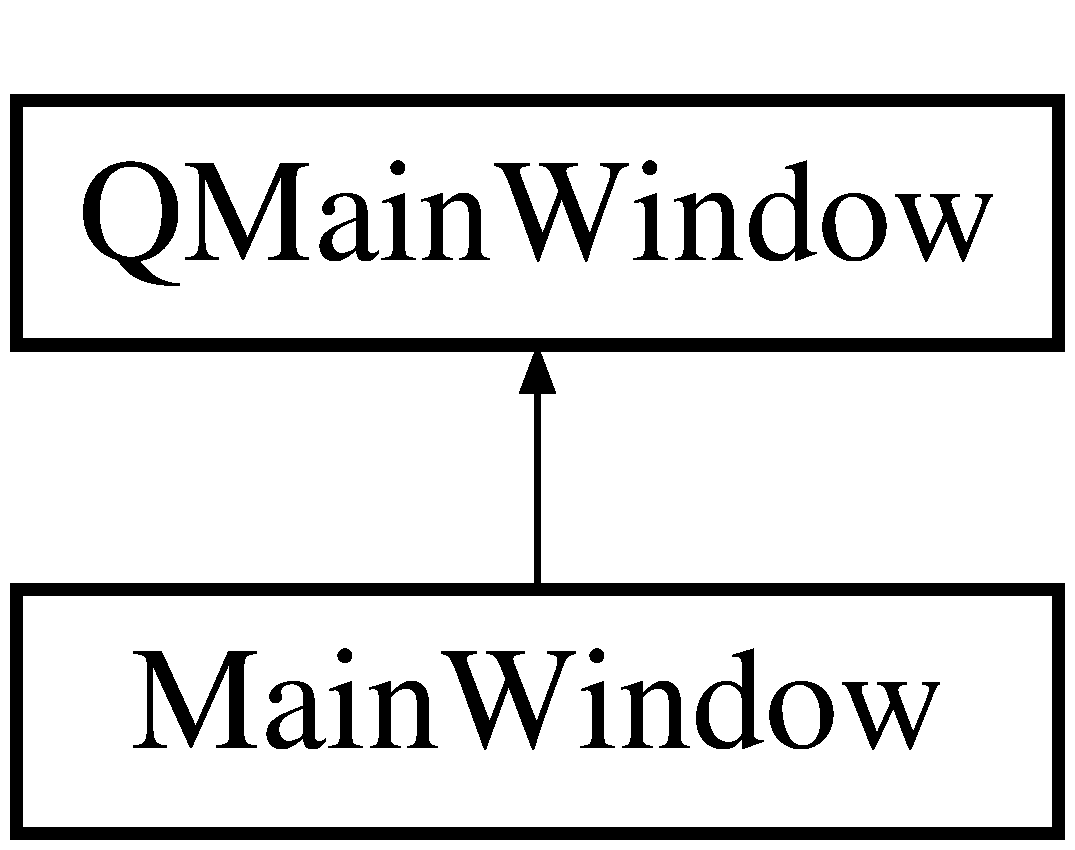
\includegraphics[height=2.000000cm]{class_main_window}
\end{center}
\end{figure}
\subsection*{Public Member Functions}
\begin{DoxyCompactItemize}
\item 
\hyperlink{class_main_window_a8b244be8b7b7db1b08de2a2acb9409db}{Main\-Window} (Q\-Widget $\ast$parent=0)
\item 
\hyperlink{class_main_window_ae98d00a93bc118200eeef9f9bba1dba7}{$\sim$\-Main\-Window} ()
\begin{DoxyCompactList}\small\item\em \hyperlink{class_main_window_ae98d00a93bc118200eeef9f9bba1dba7}{Main\-Window\-::$\sim$\-Main\-Window} Closes the U\-I window once the application is exited. \end{DoxyCompactList}\end{DoxyCompactItemize}
\subsection*{Public Attributes}
\begin{DoxyCompactItemize}
\item 
\hyperlink{class_game}{Game} \hyperlink{class_main_window_a508d487e6a6e565884e8376d6583df10}{game}
\item 
\hyperlink{class_a_i}{A\-I} \hyperlink{class_main_window_a30196d7709d113dbd8262e67e7c629e2}{computer}
\item 
int \hyperlink{class_main_window_ac8f0a233fbd35200774024901d525b25}{player\-Turn}
\end{DoxyCompactItemize}


\subsection{Detailed Description}
The \hyperlink{class_main_window}{Main\-Window} class The \hyperlink{class_main_window}{Main\-Window} class inherits the Q\-Main\-Window public class. 

This class contains the U\-I's objects and their declarations, while also containing some of the game's objects like the player's turn

class is part of the \hyperlink{namespace_ui}{Ui} namespace 

\subsection{Constructor \& Destructor Documentation}
\hypertarget{class_main_window_a8b244be8b7b7db1b08de2a2acb9409db}{\index{Main\-Window@{Main\-Window}!Main\-Window@{Main\-Window}}
\index{Main\-Window@{Main\-Window}!MainWindow@{Main\-Window}}
\subsubsection[{Main\-Window}]{\setlength{\rightskip}{0pt plus 5cm}Main\-Window\-::\-Main\-Window (
\begin{DoxyParamCaption}
\item[{Q\-Widget $\ast$}]{parent = {\ttfamily 0}}
\end{DoxyParamCaption}
)\hspace{0.3cm}{\ttfamily [explicit]}}}\label{class_main_window_a8b244be8b7b7db1b08de2a2acb9409db}
\hypertarget{class_main_window_ae98d00a93bc118200eeef9f9bba1dba7}{\index{Main\-Window@{Main\-Window}!$\sim$\-Main\-Window@{$\sim$\-Main\-Window}}
\index{$\sim$\-Main\-Window@{$\sim$\-Main\-Window}!MainWindow@{Main\-Window}}
\subsubsection[{$\sim$\-Main\-Window}]{\setlength{\rightskip}{0pt plus 5cm}Main\-Window\-::$\sim$\-Main\-Window (
\begin{DoxyParamCaption}
{}
\end{DoxyParamCaption}
)}}\label{class_main_window_ae98d00a93bc118200eeef9f9bba1dba7}


\hyperlink{class_main_window_ae98d00a93bc118200eeef9f9bba1dba7}{Main\-Window\-::$\sim$\-Main\-Window} Closes the U\-I window once the application is exited. 



\subsection{Member Data Documentation}
\hypertarget{class_main_window_a30196d7709d113dbd8262e67e7c629e2}{\index{Main\-Window@{Main\-Window}!computer@{computer}}
\index{computer@{computer}!MainWindow@{Main\-Window}}
\subsubsection[{computer}]{\setlength{\rightskip}{0pt plus 5cm}{\bf A\-I} Main\-Window\-::computer}}\label{class_main_window_a30196d7709d113dbd8262e67e7c629e2}
\hypertarget{class_main_window_a508d487e6a6e565884e8376d6583df10}{\index{Main\-Window@{Main\-Window}!game@{game}}
\index{game@{game}!MainWindow@{Main\-Window}}
\subsubsection[{game}]{\setlength{\rightskip}{0pt plus 5cm}{\bf Game} Main\-Window\-::game}}\label{class_main_window_a508d487e6a6e565884e8376d6583df10}
\hypertarget{class_main_window_ac8f0a233fbd35200774024901d525b25}{\index{Main\-Window@{Main\-Window}!player\-Turn@{player\-Turn}}
\index{player\-Turn@{player\-Turn}!MainWindow@{Main\-Window}}
\subsubsection[{player\-Turn}]{\setlength{\rightskip}{0pt plus 5cm}int Main\-Window\-::player\-Turn}}\label{class_main_window_ac8f0a233fbd35200774024901d525b25}


The documentation for this class was generated from the following files\-:\begin{DoxyCompactItemize}
\item 
\hyperlink{mainwindow_8h}{mainwindow.\-h}\item 
\hyperlink{mainwindow_8cpp}{mainwindow.\-cpp}\end{DoxyCompactItemize}

\hypertarget{struct_a_i_1_1moves}{\section{A\-I\-:\-:moves Struct Reference}
\label{struct_a_i_1_1moves}\index{A\-I\-::moves@{A\-I\-::moves}}
}


The moves struct \begin{DoxyVerb} contains the constant character values of the currentPosition, the newPositions, and the number of jumps\end{DoxyVerb}
.  




{\ttfamily \#include $<$ai.\-h$>$}

\subsection*{Public Attributes}
\begin{DoxyCompactItemize}
\item 
const char $\ast$ \hyperlink{struct_a_i_1_1moves_a736739fad02c378d6fd467d5eaf0926d}{current\-Position}
\item 
const char $\ast$ \hyperlink{struct_a_i_1_1moves_a1a70af16b28de0cb7d83c07b6663c647}{new\-Positions} \mbox{[}4\mbox{]}
\item 
const char $\ast$ \hyperlink{struct_a_i_1_1moves_a243ff8ab759ff66204e2d2152851fa65}{jumps} \mbox{[}4\mbox{]}
\end{DoxyCompactItemize}


\subsection{Detailed Description}
The moves struct \begin{DoxyVerb} contains the constant character values of the currentPosition, the newPositions, and the number of jumps\end{DoxyVerb}
. 

Definition at line 49 of file ai.\-h.



\subsection{Member Data Documentation}
\hypertarget{struct_a_i_1_1moves_a736739fad02c378d6fd467d5eaf0926d}{\index{A\-I\-::moves@{A\-I\-::moves}!current\-Position@{current\-Position}}
\index{current\-Position@{current\-Position}!AI::moves@{A\-I\-::moves}}
\subsubsection[{current\-Position}]{\setlength{\rightskip}{0pt plus 5cm}const char$\ast$ A\-I\-::moves\-::current\-Position}}\label{struct_a_i_1_1moves_a736739fad02c378d6fd467d5eaf0926d}


Definition at line 50 of file ai.\-h.

\hypertarget{struct_a_i_1_1moves_a243ff8ab759ff66204e2d2152851fa65}{\index{A\-I\-::moves@{A\-I\-::moves}!jumps@{jumps}}
\index{jumps@{jumps}!AI::moves@{A\-I\-::moves}}
\subsubsection[{jumps}]{\setlength{\rightskip}{0pt plus 5cm}const char$\ast$ A\-I\-::moves\-::jumps\mbox{[}4\mbox{]}}}\label{struct_a_i_1_1moves_a243ff8ab759ff66204e2d2152851fa65}


Definition at line 52 of file ai.\-h.

\hypertarget{struct_a_i_1_1moves_a1a70af16b28de0cb7d83c07b6663c647}{\index{A\-I\-::moves@{A\-I\-::moves}!new\-Positions@{new\-Positions}}
\index{new\-Positions@{new\-Positions}!AI::moves@{A\-I\-::moves}}
\subsubsection[{new\-Positions}]{\setlength{\rightskip}{0pt plus 5cm}const char$\ast$ A\-I\-::moves\-::new\-Positions\mbox{[}4\mbox{]}}}\label{struct_a_i_1_1moves_a1a70af16b28de0cb7d83c07b6663c647}


Definition at line 51 of file ai.\-h.



The documentation for this struct was generated from the following file\-:\begin{DoxyCompactItemize}
\item 
340\-Checkers/\hyperlink{ai_8h}{ai.\-h}\end{DoxyCompactItemize}

\hypertarget{structsq}{\section{sq Struct Reference}
\label{structsq}\index{sq@{sq}}
}


The color enum

A structure containing the values of a square, which include its x and y position and the color of the square.  




{\ttfamily \#include $<$board.\-h$>$}

\subsection*{Public Attributes}
\begin{DoxyCompactItemize}
\item 
int \hyperlink{structsq_aed5c1efc6e43c1bf7a230b8b8a373368}{x}
\item 
int \hyperlink{structsq_a1b0e5a26db37d818cb634406f2314293}{y}
\item 
int \hyperlink{structsq_a9456cfcbc3cb1beec5d3254091afa355}{color}
\end{DoxyCompactItemize}


\subsection{Detailed Description}
The color enum

A structure containing the values of a square, which include its x and y position and the color of the square. 

\subsection{Member Data Documentation}
\hypertarget{structsq_a9456cfcbc3cb1beec5d3254091afa355}{\index{sq@{sq}!color@{color}}
\index{color@{color}!sq@{sq}}
\subsubsection[{color}]{\setlength{\rightskip}{0pt plus 5cm}int sq\-::color}}\label{structsq_a9456cfcbc3cb1beec5d3254091afa355}
\hypertarget{structsq_aed5c1efc6e43c1bf7a230b8b8a373368}{\index{sq@{sq}!x@{x}}
\index{x@{x}!sq@{sq}}
\subsubsection[{x}]{\setlength{\rightskip}{0pt plus 5cm}int sq\-::x}}\label{structsq_aed5c1efc6e43c1bf7a230b8b8a373368}
\hypertarget{structsq_a1b0e5a26db37d818cb634406f2314293}{\index{sq@{sq}!y@{y}}
\index{y@{y}!sq@{sq}}
\subsubsection[{y}]{\setlength{\rightskip}{0pt plus 5cm}int sq\-::y}}\label{structsq_a1b0e5a26db37d818cb634406f2314293}


The documentation for this struct was generated from the following file\-:\begin{DoxyCompactItemize}
\item 
\hyperlink{board_8h}{board.\-h}\end{DoxyCompactItemize}

\hypertarget{classtile}{\section{tile Class Reference}
\label{classtile}\index{tile@{tile}}
}


{\ttfamily \#include $<$tile.\-h$>$}

Inheritance diagram for tile\-:\begin{figure}[H]
\begin{center}
\leavevmode
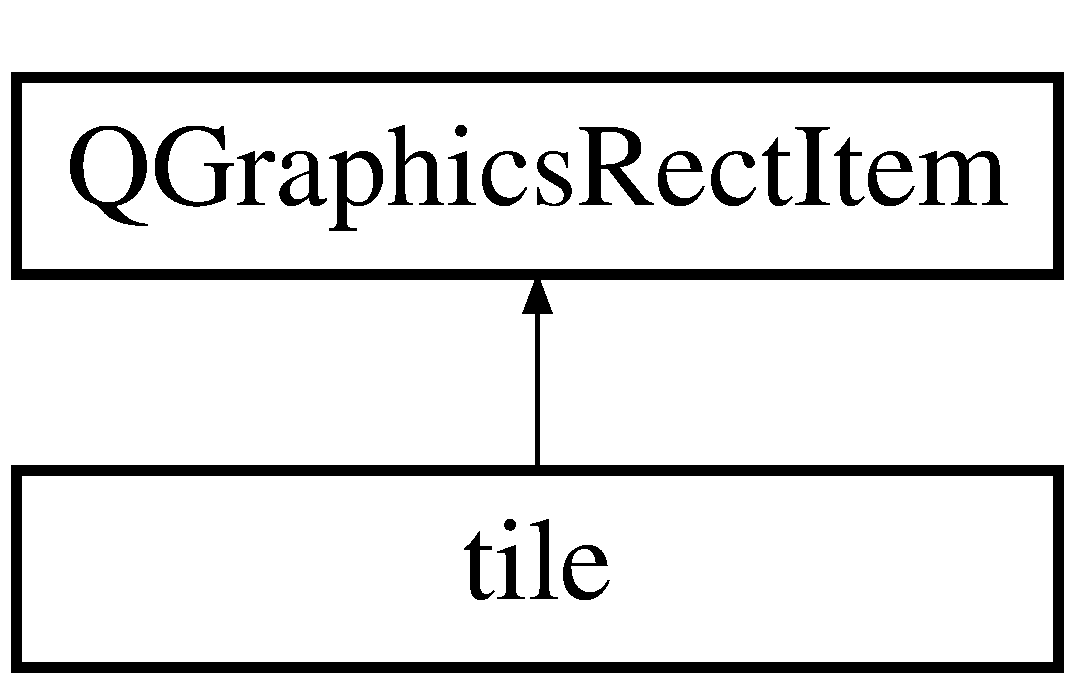
\includegraphics[height=2.000000cm]{classtile}
\end{center}
\end{figure}


The documentation for this class was generated from the following files\-:\begin{DoxyCompactItemize}
\item 
\hyperlink{tile_8h}{tile.\-h}\item 
\hyperlink{tile_8cpp}{tile.\-cpp}\end{DoxyCompactItemize}

\chapter{File Documentation}
\hypertarget{ai_8cpp}{\section{ai.\-cpp File Reference}
\label{ai_8cpp}\index{ai.\-cpp@{ai.\-cpp}}
}
{\ttfamily \#include \char`\"{}ai.\-h\char`\"{}}\\*
{\ttfamily \#include $<$iostream$>$}\\*
{\ttfamily \#include $<$string.\-h$>$}\\*
{\ttfamily \#include $<$sstream$>$}\\*
{\ttfamily \#include $<$time.\-h$>$}\\*
{\ttfamily \#include $<$stdlib.\-h$>$}\\*
\subsection*{Namespaces}
\begin{DoxyCompactItemize}
\item 
\hyperlink{namespacestd}{std}
\end{DoxyCompactItemize}


\subsection{Detailed Description}
The \hyperlink{ai_8cpp}{ai.\-cpp} file contains all of the information that deals with the A.\-I. player.

It references the classes and objects that are used and defined in the \hyperlink{game_8h}{game.\-h} file

\begin{DoxyAuthor}{Author}
Andrew Guillen 

Shane Lopez 

Kendall Zettlmeier 
\end{DoxyAuthor}
\begin{DoxyVersion}{Version}
1.\-0 
\end{DoxyVersion}

\hypertarget{ai_8h}{\section{ai.\-h File Reference}
\label{ai_8h}\index{ai.\-h@{ai.\-h}}
}
{\ttfamily \#include \char`\"{}game.\-h\char`\"{}}\\*
{\ttfamily \#include $<$vector$>$}\\*
{\ttfamily \#include $<$string.\-h$>$}\\*
{\ttfamily \#include $<$iostream$>$}\\*
\subsection*{Classes}
\begin{DoxyCompactItemize}
\item 
class \hyperlink{class_a_i}{A\-I}
\begin{DoxyCompactList}\small\item\em The \hyperlink{class_a_i}{A\-I} class. \end{DoxyCompactList}\item 
struct \hyperlink{struct_a_i_1_1moves}{A\-I\-::moves}
\begin{DoxyCompactList}\small\item\em The moves struct \begin{DoxyVerb} contains the constant character values of the currentPosition, the newPositions, and the number of jumps\end{DoxyVerb}
. \end{DoxyCompactList}\end{DoxyCompactItemize}
\subsection*{Namespaces}
\begin{DoxyCompactItemize}
\item 
\hyperlink{namespacestd}{std}
\end{DoxyCompactItemize}


\subsection{Detailed Description}
A header file that contains the objects for the \hyperlink{ai_8cpp}{ai.\-cpp} file

This contains the methods that the \hyperlink{class_a_i}{A\-I} runs when checking the moves and creating its moves. It also contains the structure for the types of moves, such as\-: the current position, a new possible position, and the number of possible jumps.

\begin{DoxyAuthor}{Author}
Andrew Guillen 

Shane Lopez 

Kendall Zettlmeier 
\end{DoxyAuthor}
\begin{DoxyVersion}{Version}
1.\-0 
\end{DoxyVersion}

\hypertarget{board_8cpp}{\section{340\-Checkers/board.cpp File Reference}
\label{board_8cpp}\index{340\-Checkers/board.\-cpp@{340\-Checkers/board.\-cpp}}
}
{\ttfamily \#include \char`\"{}board.\-h\char`\"{}}\\*
{\ttfamily \#include $<$iostream$>$}\\*
\subsection*{Namespaces}
\begin{DoxyCompactItemize}
\item 
\hyperlink{namespacestd}{std}
\end{DoxyCompactItemize}


\subsection{Detailed Description}
This is where the board is initialized.

This contains everything that the board does, from initially generating the board to properly displaying the current board status (which is the current move). It is constantly refreshed whenever a new move is made.

\begin{DoxyAuthor}{Author}
Andrew Guillen 

Shane Lopez 

Kendall Zettlmeier 
\end{DoxyAuthor}
\begin{DoxyVersion}{Version}
1.\-0
\end{DoxyVersion}
\begin{DoxyRefDesc}{Bug}
\item[\hyperlink{bug__bug000002}{Bug}]No bugs were found with testing. \end{DoxyRefDesc}


Definition in file \hyperlink{board_8cpp_source}{board.\-cpp}.


\hypertarget{board_8h}{\section{board.\-h File Reference}
\label{board_8h}\index{board.\-h@{board.\-h}}
}
{\ttfamily \#include $<$Q\-Graphics\-Scene$>$}\\*
{\ttfamily \#include $<$Qt\-Gui$>$}\\*
{\ttfamily \#include $<$unistd.\-h$>$}\\*
\subsection*{Classes}
\begin{DoxyCompactItemize}
\item 
struct \hyperlink{structsq}{sq}
\begin{DoxyCompactList}\small\item\em The color enum

A structure containing the values of a square, which include its x and y position and the color of the square. \end{DoxyCompactList}\item 
class \hyperlink{class_board}{Board}
\end{DoxyCompactItemize}
\subsection*{Macros}
\begin{DoxyCompactItemize}
\item 
\#define \hyperlink{board_8h_a8e24a27ddbc8df73d255819cff590c78}{S\-Q\-\_\-\-S}~40
\end{DoxyCompactItemize}
\subsection*{Typedefs}
\begin{DoxyCompactItemize}
\item 
typedef struct \hyperlink{structsq}{sq} \hyperlink{board_8h_a07a2313fe921ff279f333a9888a9f197}{sq}
\end{DoxyCompactItemize}
\subsection*{Enumerations}
\begin{DoxyCompactItemize}
\item 
enum \hyperlink{board_8h_a37dbdc30935031c05304482e1be89d8f}{color} \{ \hyperlink{board_8h_a37dbdc30935031c05304482e1be89d8faf80f9a890089d211842d59625e561f88}{R\-E\-D}, 
\hyperlink{board_8h_a37dbdc30935031c05304482e1be89d8faf77fb67151d0c18d397069ad8c271ba3}{B\-L\-A\-C\-K}
 \}
\end{DoxyCompactItemize}


\subsection{Detailed Description}
The board header file

This is the board header file, this is where the board will be stored. This also store the board length, in which if you wanted a bigger board you can do it here. This is also where we have the display board function, which was was used to create the checkers game as a console application.

\begin{DoxyAuthor}{Author}
Andrew Guillen 

Shane Lopez 

Kendall Zettlmeier 
\end{DoxyAuthor}
\begin{DoxyVersion}{Version}
1.\-0 
\end{DoxyVersion}


\subsection{Macro Definition Documentation}
\hypertarget{board_8h_a8e24a27ddbc8df73d255819cff590c78}{\index{board.\-h@{board.\-h}!S\-Q\-\_\-\-S@{S\-Q\-\_\-\-S}}
\index{S\-Q\-\_\-\-S@{S\-Q\-\_\-\-S}!board.h@{board.\-h}}
\subsubsection[{S\-Q\-\_\-\-S}]{\setlength{\rightskip}{0pt plus 5cm}\#define S\-Q\-\_\-\-S~40}}\label{board_8h_a8e24a27ddbc8df73d255819cff590c78}
Pre-\/defines the size of the square to about 40 pixels 

\subsection{Typedef Documentation}
\hypertarget{board_8h_a07a2313fe921ff279f333a9888a9f197}{\index{board.\-h@{board.\-h}!sq@{sq}}
\index{sq@{sq}!board.h@{board.\-h}}
\subsubsection[{sq}]{\setlength{\rightskip}{0pt plus 5cm}typedef struct {\bf sq} {\bf sq}}}\label{board_8h_a07a2313fe921ff279f333a9888a9f197}


\subsection{Enumeration Type Documentation}
\hypertarget{board_8h_a37dbdc30935031c05304482e1be89d8f}{\index{board.\-h@{board.\-h}!color@{color}}
\index{color@{color}!board.h@{board.\-h}}
\subsubsection[{color}]{\setlength{\rightskip}{0pt plus 5cm}enum {\bf color}}}\label{board_8h_a37dbdc30935031c05304482e1be89d8f}
\begin{Desc}
\item[Enumerator]\par
\begin{description}
\index{R\-E\-D@{R\-E\-D}!board.\-h@{board.\-h}}\index{board.\-h@{board.\-h}!R\-E\-D@{R\-E\-D}}\item[{\em 
\hypertarget{board_8h_a37dbdc30935031c05304482e1be89d8faf80f9a890089d211842d59625e561f88}{R\-E\-D}\label{board_8h_a37dbdc30935031c05304482e1be89d8faf80f9a890089d211842d59625e561f88}
}]\index{B\-L\-A\-C\-K@{B\-L\-A\-C\-K}!board.\-h@{board.\-h}}\index{board.\-h@{board.\-h}!B\-L\-A\-C\-K@{B\-L\-A\-C\-K}}\item[{\em 
\hypertarget{board_8h_a37dbdc30935031c05304482e1be89d8faf77fb67151d0c18d397069ad8c271ba3}{B\-L\-A\-C\-K}\label{board_8h_a37dbdc30935031c05304482e1be89d8faf77fb67151d0c18d397069ad8c271ba3}
}]\end{description}
\end{Desc}

\hypertarget{game_8cpp}{\section{340\-Checkers/game.cpp File Reference}
\label{game_8cpp}\index{340\-Checkers/game.\-cpp@{340\-Checkers/game.\-cpp}}
}


\hyperlink{class_game}{Game} Logic implementation.  


{\ttfamily \#include \char`\"{}game.\-h\char`\"{}}\\*
{\ttfamily \#include $<$iostream$>$}\\*
{\ttfamily \#include $<$sstream$>$}\\*
\subsection*{Namespaces}
\begin{DoxyCompactItemize}
\item 
\hyperlink{namespacestd}{std}
\end{DoxyCompactItemize}


\subsection{Detailed Description}
\hyperlink{class_game}{Game} Logic implementation. All game logic is coded here. It contains the information for keeping track of moves for both players, whether or not a player is the C\-P\-U or not. It receives information of where a player wants to commit their move and properly insepcts their commitment to see if a given move attempt is legal.

\begin{DoxyAuthor}{Author}
Andrew Guillen 

Shane Lopez 

Kendall Zettlmeier 
\end{DoxyAuthor}
\begin{DoxyVersion}{Version}
1.\-0
\end{DoxyVersion}
\begin{DoxyRefDesc}{Bug}
\item[\hyperlink{bug__bug000004}{Bug}]No major bugs found other than the bug specified on the \hyperlink{ai_8cpp}{A\-I.\-cpp} file \end{DoxyRefDesc}


Definition in file \hyperlink{game_8cpp_source}{game.\-cpp}.


\hypertarget{game_8h}{\section{340\-Checkers/game.h File Reference}
\label{game_8h}\index{340\-Checkers/game.\-h@{340\-Checkers/game.\-h}}
}
{\ttfamily \#include \char`\"{}board.\-h\char`\"{}}\\*
{\ttfamily \#include $<$string.\-h$>$}\\*
{\ttfamily \#include $<$iostream$>$}\\*
\subsection*{Classes}
\begin{DoxyCompactItemize}
\item 
class \hyperlink{class_game}{Game}
\end{DoxyCompactItemize}
\subsection*{Namespaces}
\begin{DoxyCompactItemize}
\item 
\hyperlink{namespacestd}{std}
\end{DoxyCompactItemize}


\subsection{Detailed Description}
The game header file

This is the place where all of the current pieces from the game board are stored; it also includes the scores of eacher player, which indicates how many pieces a player has left on the board. All of the methods that are required for the game logic are stored in this file as well. It makes it much easier to maintain the information for the games moves here rather than keeping the information with the computational parts of the application.

\begin{DoxyAuthor}{Author}
Andrew Guillen 

Shane Lopez 

Kendall Zettlmeier 
\end{DoxyAuthor}
\begin{DoxyVersion}{Version}
1.\-0 
\end{DoxyVersion}
\begin{DoxyRefDesc}{Bug}
\item[\hyperlink{bug__bug000005}{Bug}]No bugs have been spotted.\end{DoxyRefDesc}


Definition in file \hyperlink{game_8h_source}{game.\-h}.


\hypertarget{main_8cpp}{\section{340\-Checkers/main.cpp File Reference}
\label{main_8cpp}\index{340\-Checkers/main.\-cpp@{340\-Checkers/main.\-cpp}}
}


This is the main class that starts the application.  


{\ttfamily \#include \char`\"{}mainwindow.\-h\char`\"{}}\\*
{\ttfamily \#include $<$Q\-Application$>$}\\*
\subsection*{Functions}
\begin{DoxyCompactItemize}
\item 
int \hyperlink{main_8cpp_a0ddf1224851353fc92bfbff6f499fa97}{main} (int argc, char $\ast$argv\mbox{[}$\,$\mbox{]})
\begin{DoxyCompactList}\small\item\em main The main function of the application \end{DoxyCompactList}\end{DoxyCompactItemize}


\subsection{Detailed Description}
This is the main class that starts the application. This will start up the application and start up the game.

\begin{DoxyAuthor}{Author}
Andrew Guillen 

Shane Lopez 

Kendall Zettlmeier 
\end{DoxyAuthor}
\begin{DoxyVersion}{Version}
1.\-0 
\end{DoxyVersion}
\begin{DoxyDate}{Date}
December 2013 
\end{DoxyDate}
\begin{DoxyRefDesc}{Bug}
\item[\hyperlink{bug__bug000006}{Bug}]No major bugs were found upon testing \end{DoxyRefDesc}
\begin{DoxyWarning}{Warning}
If your computer does not contain the standard C libraries, such as 'stdlib.\-h', then the application may not run. 
\end{DoxyWarning}


Definition in file \hyperlink{main_8cpp_source}{main.\-cpp}.



\subsection{Function Documentation}
\hypertarget{main_8cpp_a0ddf1224851353fc92bfbff6f499fa97}{\index{main.\-cpp@{main.\-cpp}!main@{main}}
\index{main@{main}!main.cpp@{main.\-cpp}}
\subsubsection[{main}]{\setlength{\rightskip}{0pt plus 5cm}int main (
\begin{DoxyParamCaption}
\item[{int}]{argc, }
\item[{char $\ast$}]{argv\mbox{[}$\,$\mbox{]}}
\end{DoxyParamCaption}
)}}\label{main_8cpp_a0ddf1224851353fc92bfbff6f499fa97}


main The main function of the application 


\begin{DoxyParams}{Parameters}
{\em argc} & The argument counter (used initially for the command line variation of the checkers game) \\
\hline
{\em argv} & The argument vector pointing to the command line arguments themselves \\
\hline
\end{DoxyParams}
\begin{DoxyReturn}{Returns}
The U\-I window opened with the application running 
\end{DoxyReturn}
a \begin{DoxyReturn}{Returns}

\end{DoxyReturn}


Definition at line 29 of file main.\-cpp.


\hypertarget{mainwindow_8cpp}{\section{340\-Checkers/mainwindow.cpp File Reference}
\label{mainwindow_8cpp}\index{340\-Checkers/mainwindow.\-cpp@{340\-Checkers/mainwindow.\-cpp}}
}
{\ttfamily \#include \char`\"{}mainwindow.\-h\char`\"{}}\\*
{\ttfamily \#include \char`\"{}ui\-\_\-mainwindow.\-h\char`\"{}}\\*
{\ttfamily \#include $<$iostream$>$}\\*
{\ttfamily \#include $<$stdlib.\-h$>$}\\*
\subsection*{Namespaces}
\begin{DoxyCompactItemize}
\item 
\hyperlink{namespacestd}{std}
\end{DoxyCompactItemize}


\subsection{Detailed Description}
The main interface of the U\-I

This is where the U\-I does its work. It is used to start the game, make the moves and quitting the application. Most of what the U\-I has to access, such as signals, slots, and widgets are located here.

\begin{DoxyAuthor}{Author}
Andrew Guillen 

Shane Lopez 

Kendall Zettlmeier 
\end{DoxyAuthor}
\begin{DoxyVersion}{Version}
1.\-0 
\end{DoxyVersion}
\begin{DoxyDate}{Date}
December 2013 
\end{DoxyDate}
\begin{DoxyRefDesc}{Bug}
\item[\hyperlink{bug__bug000007}{Bug}]No major bugs were found upon testing\end{DoxyRefDesc}


Definition in file \hyperlink{mainwindow_8cpp_source}{mainwindow.\-cpp}.


\hypertarget{mainwindow_8h}{\section{mainwindow.\-h File Reference}
\label{mainwindow_8h}\index{mainwindow.\-h@{mainwindow.\-h}}
}
{\ttfamily \#include $<$Q\-Main\-Window$>$}\\*
{\ttfamily \#include $<$Q\-Graphics\-Scene$>$}\\*
{\ttfamily \#include $<$Q\-Graphics\-View$>$}\\*
{\ttfamily \#include \char`\"{}game.\-h\char`\"{}}\\*
{\ttfamily \#include \char`\"{}ai.\-h\char`\"{}}\\*
\subsection*{Classes}
\begin{DoxyCompactItemize}
\item 
class \hyperlink{class_main_window}{Main\-Window}
\begin{DoxyCompactList}\small\item\em The \hyperlink{class_main_window}{Main\-Window} class The \hyperlink{class_main_window}{Main\-Window} class inherits the Q\-Main\-Window public class. \end{DoxyCompactList}\end{DoxyCompactItemize}
\subsection*{Namespaces}
\begin{DoxyCompactItemize}
\item 
\hyperlink{namespace_ui}{Ui}
\end{DoxyCompactItemize}


\subsection{Detailed Description}
Header file for the U\-I

This is the header file for the U\-I. It includes all of the objects that the U\-I is in charge of and all of the objects that are used by the U\-I are stored in this file. The current player's turn and some game objects are declared here, since we felt it was necessary.

\begin{DoxyAuthor}{Author}
Andrew Guillen 

Shane Lopez 

Kendall Zettlmeier 
\end{DoxyAuthor}
\begin{DoxyVersion}{Version}
1.\-0 
\end{DoxyVersion}
\begin{DoxyDate}{Date}
December 2013 
\end{DoxyDate}
\begin{DoxyRefDesc}{Bug}
\item[\hyperlink{bug__bug000004}{Bug}]No major bugs were found upon testing\end{DoxyRefDesc}

\hypertarget{tile_8cpp}{\section{tile.\-cpp File Reference}
\label{tile_8cpp}\index{tile.\-cpp@{tile.\-cpp}}
}
{\ttfamily \#include \char`\"{}tile.\-h\char`\"{}}\\*


\subsection{Detailed Description}
Contains the actions for the U\-I events

This creates the tiles that populate the grid and create a graphical representation of the checker board. This depicts the same game logic and moves that are calculated in the other files, but shows a visual representation of casting a player's move and moving the piece to a new valid location on the board.

\begin{DoxyAuthor}{Author}
Andrew Guillen 

Shane Lopez 

Kendall Zettlmeier 
\end{DoxyAuthor}
\begin{DoxyVersion}{Version}
1.\-0 
\end{DoxyVersion}
\begin{DoxyDate}{Date}
December 2013 
\end{DoxyDate}
\begin{DoxyRefDesc}{Bug}
\item[\hyperlink{bug__bug000005}{Bug}]No major bugs were found upon testing\end{DoxyRefDesc}

\hypertarget{tile_8h}{\section{340\-Checkers/tile.h File Reference}
\label{tile_8h}\index{340\-Checkers/tile.\-h@{340\-Checkers/tile.\-h}}
}
{\ttfamily \#include $<$Qt\-Gui$>$}\\*
{\ttfamily \#include $<$Q\-Graphics\-Rect\-Item$>$}\\*
\subsection*{Classes}
\begin{DoxyCompactItemize}
\item 
class \hyperlink{classtile}{tile}
\end{DoxyCompactItemize}
\subsection*{Macros}
\begin{DoxyCompactItemize}
\item 
\#define \hyperlink{tile_8h_af933676109efed7ab34cea71d748a517}{S}~40
\end{DoxyCompactItemize}


\subsection{Detailed Description}
Tile header file

This header file contains the objects that are used by the \hyperlink{tile_8cpp}{tile.\-cpp} file that display the spots on the board.

\begin{DoxyAuthor}{Author}
Andrew Guillen 

Shane Lopez 

Kendall Zettlmeier 
\end{DoxyAuthor}
\begin{DoxyVersion}{Version}
1.\-0 
\end{DoxyVersion}
\begin{DoxyDate}{Date}
December 2013 
\end{DoxyDate}
\begin{DoxyRefDesc}{Bug}
\item[\hyperlink{bug__bug000010}{Bug}]No major bugs were found upon testing\end{DoxyRefDesc}


Definition in file \hyperlink{tile_8h_source}{tile.\-h}.



\subsection{Macro Definition Documentation}
\hypertarget{tile_8h_af933676109efed7ab34cea71d748a517}{\index{tile.\-h@{tile.\-h}!S@{S}}
\index{S@{S}!tile.h@{tile.\-h}}
\subsubsection[{S}]{\setlength{\rightskip}{0pt plus 5cm}\#define S~40}}\label{tile_8h_af933676109efed7ab34cea71d748a517}


Definition at line 24 of file tile.\-h.


%--- End generated contents ---

% Index
\newpage
\phantomsection
\addcontentsline{toc}{part}{Index}
\printindex

\end{document}
